%
%%%%%%%%%%%%%%%%%%%%%%%%%%%%%%%%%%%%%%%%%%%%%%%%%%%%%%%%%%%%%%%%%%%%%%
%%                                                                 %%
%% Please do not use \input{...} to include other tex files.       %%
%% Submit your LaTeX manuscript as one .tex document.              %%
%%                                                                 %%
%% All additional figures and files should be attached             %%
%% separately and not embedded in the \TeX\ document itself.       %%
%%                                                                 %%
%%%%%%%%%%%%%%%%%%%%%%%%%%%%%%%%%%%%%%%%%%%%%%%%%%%%%%%%%%%%%%%%%%%%%

%%\documentclass[referee,sn-basic]{sn-jnl}% referee option is meant for double line spacing

%%=======================================================%%
%% to print line numbers in the margin use lineno option %%
%%=======================================================%%

%%\documentclass[lineno,pdflatex,sn-basic]{sn-jnl}% Basic Springer Nature Reference Style/Chemistry Reference Style

%%=========================================================================================%%
%% the documentclass is set to pdflatex as default. You can delete it if not appropriate.  %%
%%=========================================================================================%%

%%\documentclass[sn-basic]{sn-jnl}% Basic Springer Nature Reference Style/Chemistry Reference Style

%%Note: the following reference styles support Namedate and Numbered referencing. By default the style follows the most common style. To switch between the options you can add or remove “Numbered” in the optional parenthesis. 
%%The option is available for: sn-basic.bst, sn-chicago.bst%  
 
%%\documentclass[pdflatex,sn-nature]{sn-jnl}% Style for submissions to Nature Portfolio journals
%%\documentclass[pdflatex,sn-basic]{sn-jnl}% Basic Springer Nature Reference Style/Chemistry Reference Style
\documentclass[pdflatex,sn-mathphys-num]{sn-jnl}% Math and Physical Sciences Numbered Reference Style
%%\documentclass[pdflatex,sn-mathphys-ay]{sn-jnl}% Math and Physical Sciences Author Year Reference Style
%%\documentclass[pdflatex,sn-aps]{sn-jnl}% American Physical Society (APS) Reference Style
%%\documentclass[pdflatex,sn-vancouver-num]{sn-jnl}% Vancouver Numbered Reference Style
%%\documentclass[pdflatex,sn-vancouver-ay]{sn-jnl}% Vancouver Author Year Reference Style
%%\documentclass[pdflatex,sn-apa]{sn-jnl}% APA Reference Style
%%\documentclass[pdflatex,sn-chicago]{sn-jnl}% Chicago-based Humanities Reference Style

%%%% Standard Packages
%%<additional latex packages if required can be included here>

\usepackage{graphicx}%
\usepackage{multirow}%
\usepackage{amsmath,amssymb,amsfonts}%
\usepackage{amsthm}%
\usepackage{mathrsfs}%
\usepackage[title]{appendix}%
\usepackage{xcolor}%
\usepackage{textcomp}%
\usepackage{manyfoot}%
\usepackage{booktabs}%
\usepackage{algorithm}%
\usepackage{algorithmicx}%
\usepackage{algpseudocode}%
\usepackage{listings}%
\usepackage{placeins}%
\usepackage{float}%
%%%%

%%%%%=============================================================================%%%%
%%%%  Remarks: This template is provided to aid authors with the preparation
%%%%  of original research articles intended for submission to journals published 
%%%%  by Springer Nature. The guidance has been prepared in partnership with 
%%%%  production teams to conform to Springer Nature technical requirements. 
%%%%  Editorial and presentation requirements differ among journal portfolios and 
%%%%  research disciplines. You may find sections in this template are irrelevant 
%%%%  to your work and are empowered to omit any such section if allowed by the 
%%%%  journal you intend to submit to. The submission guidelines and policies 
%%%%  of the journal take precedence. A detailed User Manual is available in the 
%%%%  template package for technical guidance.
%%%%%=============================================================================%%%%

%% as per the requirement new theorem styles can be included as shown below
\theoremstyle{thmstyleone}%
\newtheorem{theorem}{Theorem}%  meant for continuous numbers
%%\newtheorem{theorem}{Theorem}[section]% meant for sectionwise numbers
%% optional argument [theorem] produces theorem numbering sequence instead of independent numbers for Proposition
\newtheorem{proposition}[theorem]{Proposition}% 
%%\newtheorem{proposition}{Proposition}% to get separate numbers for theorem and proposition etc.

\theoremstyle{thmstyletwo}%
\newtheorem{example}{Example}%
\newtheorem{remark}{Remark}%

\theoremstyle{thmstylethree}%
\newtheorem{definition}{Definition}%

\raggedbottom
%%\unnumbered% uncomment this for unnumbered level heads

\begin{document}

\title[HPC-Accelerated Quantum Kernels]{HPC-Accelerated Quantum Kernel Simulation for Biomedical Data Analysis}

%%=============================================================%%
%% GivenName	-> \fnm{Joergen W.}
%% Particle	-> \spfx{van der} -> surname prefix
%% FamilyName	-> \sur{Ploeg}
%% Suffix	-> \sfx{IV}
%% \author*[1,2]{\fnm{Joergen W.} \spfx{van der} \sur{Ploeg} 
%%  \sfx{IV}}\email{iauthor@gmail.com}
%%=============================================================%%

\author*[1]{\fnm{Kyle} \sur{Hartness}}\email{kahartne@utica.edu}

\author[2]{\fnm{Sofia} \sur{Furda}}\email{soffurda@gmail.com}

\author[3]{\fnm{Edmund} \sur{Bombardieri}}\email{ebombardieri@mail.wlu.edu}

% Mentor authorship: confirm during final project meeting before enabling.
\author[4]{\fnm{Rutal} \sur{Mahajan}}\email{rutal.mahajan@gmail.com}
% If mentor is an author, removes from acknowledgements and instead add the following into contributions:

% Rutal Mahajan supervised the project, provided research guidance, and advised
% the development and evaluation of the HPC benchmarking methodology.


\affil*[1]{\orgname{Utica University}, \orgaddress{\city{Utica}, \state{NY}, \country{USA}}}

% Sofia institutional affiliation
\affil[2]{\orgname{Pace University}, \orgaddress{\city{New York}, \state{NY}, \country{USA}}}

% Edmund affiliation
\affil[3]{\orgname{Washington and Lee University}, \orgaddress{\city{Lexington City}, \state{Virginia}, \country{USA}}}

% TODO: Add mentor affiliation if added as author

%%==================================%%
%% Sample for unstructured abstract %%
%%==================================%%

\abstract{
Quantum-kernel methods provide a mechanism for embedding classical data into
quantum state spaces, but classical simulation of quantum circuits becomes
increasingly expensive as circuit size and workload scale. This work develops
and evaluates a high-performance computing workflow for quantum-kernel
simulation using a biomedical electromyography workload derived from the
NinaPro DB2 dataset. Surface-EMG recordings were processed into 36 classical
features and reduced to eight quantum input features for an eight-qubit,
manually constructed ZZFeatureMap. A quantum kernel was then computed from
pairwise state overlaps.

The implementation was validated across local CPU and CUDA-capable GPU
simulation backends, with a maximum numerical difference of approximately
$4.77\times10^{-7}$ between the resulting kernel matrices. For the complete
$102\times102$ eight-qubit NinaPro kernel workload, the local CPU completed the
benchmark faster than the GPU, while separate qubit-scaling experiments showed that the GPU was faster at the
largest tested problem size of 16 qubits. A depolarizing-noise experiment
across five noise strengths showed a gradual reduction in mean state fidelity
while per-sample simulation runtime remained approximately constant. Final Bridges-2 strong-scaling experiments reduced mean runtime from
0.168016~s with one MPI process to 0.024862~s with eight processes,
corresponding to a speedup of approximately \(6.76\times\) and a parallel
efficiency of 84.47\%. A final full-capacity real-data experiment used
1,404 distinct non-overlapping NinaPro EMG windows, producing 986,310
quantum-kernel pairs. Mean runtime decreased from 4.198034~s with one MPI
process to 0.378437~s with 128 processes on one node. When the same 128
processes were distributed across 16 physical Bridges-2 nodes, mean runtime
decreased further to 0.365481~s, corresponding to an overall
\(11.49\times\) speedup relative to the single-process baseline. On Bridges-2, V100 statevector simulation remained approximately at CPU
performance through 14 qubits but achieved a measured \(1.067\times\)
speedup at the largest tested size of 16 qubits, while the GPU tensor-network
backend did not outperform CPU statevector simulation over the tested range. Together, these experiments establish a reproducible framework for
studying CPU, GPU, noise, and distributed-memory scaling of simulated quantum
kernel workloads on biomedical data.
}

%%================================%%
%% Sample for structured abstract %%
%%================================%%

% \abstract{\textbf{Purpose:} The abstract serves both as a general introduction to the topic and as a brief, non-technical summary of the main results and their implications. The abstract must not include subheadings (unless expressly permitted in the journal's Instructions to Authors), equations or citations. As a guide the abstract should not exceed 200 words. Most journals do not set a hard limit however authors are advised to check the author instructions for the journal they are submitting to.
% 
% \textbf{Methods:} The abstract serves both as a general introduction to the topic and as a brief, non-technical summary of the main results and their implications. The abstract must not include subheadings (unless expressly permitted in the journal's Instructions to Authors), equations or citations. As a guide the abstract should not exceed 200 words. Most journals do not set a hard limit however authors are advised to check the author instructions for the journal they are submitting to.
% 
% \textbf{Results:} The abstract serves both as a general introduction to the topic and as a brief, non-technical summary of the main results and their implications. The abstract must not include subheadings (unless expressly permitted in the journal's Instructions to Authors), equations or citations. As a guide the abstract should not exceed 200 words. Most journals do not set a hard limit however authors are advised to check the author instructions for the journal they are submitting to.
% 
% \textbf{Conclusion:} The abstract serves both as a general introduction to the topic and as a brief, non-technical summary of the main results and their implications. The abstract must not include subheadings (unless expressly permitted in the journal's Instructions to Authors), equations or citations. As a guide the abstract should not exceed 200 words. Most journals do not set a hard limit however authors are advised to check the author instructions for the journal they are submitting to.}

\keywords{
quantum computing,
quantum kernels,
high-performance computing,
MPI,
GPU acceleration,
biomedical signal processing,
electromyography,
NinaPro
}

%%\pacs[JEL Classification]{D8, H51}

%%\pacs[MSC Classification]{35A01, 65L10, 65L12, 65L20, 65L70}

\maketitle

\section{Introduction}\label{sec1}

Quantum computing provides new computational models for representing and
processing information, including approaches in which classical feature vectors
are encoded into quantum states. Quantum kernel methods use these state
representations to construct similarity measures in a quantum feature space,
allowing classical machine-learning procedures to operate on kernel matrices
derived from quantum circuits. Quantum feature maps such as the ZZFeatureMap
have therefore become an important component of quantum machine-learning
research \cite{havlicek2019}.

For near-term research, however, quantum algorithms are frequently investigated
through classical simulation rather than exclusively on physical quantum
hardware. Frameworks such as Qiskit provide programmable circuit construction,
while Qiskit Aer provides multiple classical simulation methods and configurable
noise models \cite{qiskit2024,qiskitaer2025}. Classical quantum simulation is
computationally demanding because the state space represented by a general
statevector grows exponentially with the number of qubits. This makes simulator
performance, hardware acceleration, and parallel execution important concerns
when quantum experiments are extended to larger circuits or larger collections
of independent simulations.

High-performance computing provides several mechanisms for addressing these
computational demands. CPU parallelism can accelerate independent calculations,
GPU backends can exploit highly parallel numerical hardware, and distributed-
memory programming with the Message Passing Interface (MPI) can divide larger
computational workloads across multiple processes. These approaches do not
guarantee improved performance for every problem size, because initialization,
communication, data movement, and accelerator overhead can outweigh the
benefits of parallel execution for smaller workloads. Performance must therefore
be measured experimentally across problem sizes and computing environments.

This work investigates these questions through a reproducible quantum-kernel
benchmarking workflow. The study focuses on four related objectives:
(1) validating a manually constructed quantum feature map and quantum-kernel
implementation; (2) comparing CPU and CUDA-capable GPU simulation performance;
(3) evaluating the sensitivity of simulated quantum states to controlled
depolarizing noise; and (4) characterizing distributed-memory scaling using MPI
on the Bridges-2 high-performance computing system.

To provide a real biomedical workload, the final benchmark uses surface
electromyography (sEMG) data from the NinaPro DB2 dataset. The selected data are
processed into time-domain EMG features and reduced to eight numerical inputs,
which are encoded by an eight-qubit quantum feature map. The resulting
$102\times102$ quantum kernel provides a fixed real-data workload for numerical
validation and CPU/GPU benchmarking, while the independent pairwise kernel
calculations also provide a natural unit of work for MPI distribution.

The project originated as one component of a broader DREU-QIS research effort
investigating quantum-enhanced and privacy-aware machine-learning workflows.
Within that effort, the present work addresses the HPC benchmarking and
parallelization track. Earlier development established the circuit-simulation
framework, a SLURM execution workflow on Bridges-2, and preliminary MPI scaling.
The present study extends that foundation with the NinaPro real-data workload,
local CPU/GPU validation, qubit-scaling experiments, and controlled
depolarizing-noise analysis. Final strong- and weak-scaling experiments using the 102-sample NinaPro
quantum-kernel workload were subsequently executed on Bridges-2 using
1, 2, 4, and 8 MPI processes. The distributed-memory evaluation was then
extended to matched single-node and multi-node configurations at 8, 16,
and 32 MPI processes. A larger balanced real-data workload using seven
non-overlapping windows from each gesture--repetition segment produced
714 distinct real EMG windows and 255,255 kernel pairs.

To evaluate the MPI implementation at the maximum non-overlapping-window
capacity of the selected recording, a final workload retained every complete
512-sample window available from each gesture--repetition segment. This
produced 1,404 distinct real EMG windows and 986,310 upper-triangular
quantum-kernel pairs. Process-count scaling was evaluated through 128 MPI
ranks, and physical-node scaling was evaluated by distributing 128 fixed
ranks across as many as 16 Bridges-2 Regular Memory nodes.

The primary contribution of this work is therefore not a claim of quantum
advantage or improved biomedical classification accuracy. Instead, it is an
experimental characterization of how a reproducible simulated quantum-kernel
workload behaves across CPU, GPU, noisy-simulation, and distributed HPC
configurations. This distinction is important because simulator performance and
parallel scalability are prerequisites for evaluating larger quantum
machine-learning experiments reliably.

\section{Related Work}\label{sec:related-work}

\subsection{Quantum Feature Maps and Quantum Kernels}
\label{subsec:related-quantum-kernels}

Quantum kernel methods encode classical data into quantum states and use
state-space similarity as a kernel for downstream machine-learning methods.
Havl\'{\i}\v{c}ek et al. demonstrated a quantum-enhanced feature-space
approach in which classical samples are mapped into a Hilbert space through
parameterized quantum circuits and compared using quantum-state overlaps
\cite{havlicek2019}. This framework motivates the use of quantum feature maps
as a mechanism for constructing kernel matrices from classical data.

In the present work, this general approach is used as a computational workload
rather than as evidence of quantum classification advantage. The focus is on
the cost of constructing and simulating the feature-map states and evaluating
their pairwise overlaps across different classical computing environments.


\subsection{Quantum-Circuit Simulation}
\label{subsec:related-simulation}

Practical quantum-algorithm research frequently relies on classical simulation
during development and validation. Qiskit provides a software framework for
constructing, transforming, and evaluating quantum circuits
\cite{qiskit2024}. Qiskit Aer extends this workflow with high-performance
simulation methods including statevector and density-matrix simulation, noise
models, and accelerator-capable execution \cite{qiskitaer2025}.

Classical simulation becomes increasingly expensive as the number of qubits
increases because the size of a general statevector grows exponentially with
qubit count. Simulator implementation, available memory, CPU parallelism, and
accelerator hardware therefore become important experimental considerations.
These characteristics motivate the CPU/GPU and qubit-scaling measurements used
in this study.


\subsection{High-Performance Computing and MPI}
\label{subsec:related-hpc}

The Message Passing Interface (MPI) is a standardized programming model for
distributed-memory parallel computing that enables independent processes to
coordinate computation and exchange data across processors and compute nodes
\cite{mpiforum2023,gropp2014usingmpi}.

Parallel performance is commonly characterized through strong and weak scaling.
Strong scaling measures how runtime changes as additional processing resources
are applied to a fixed total workload. Weak scaling instead increases the total
problem size with the amount of available parallel hardware in order to
evaluate whether runtime remains stable as the system scales.

The present work applies MPI at the quantum-kernel workload level. Independent
pairwise kernel calculations are distributed between ranks rather than
partitioning the internal quantum state of one circuit simulation. This design
is well suited to a kernel matrix because different matrix elements can be
computed independently before the results are combined.


\subsection{Distributed and Accelerated Quantum Simulation}
\label{subsec:related-accelerated-simulation}

Quantum simulation frameworks can also use parallel hardware internally.
Qiskit Aer supports configurable parallel execution and provides mechanisms for
GPU-accelerated and MPI-enabled simulation in supported environments
\cite{aermpi}. Such distributed simulator implementations can partition the
simulation of a single quantum state when the circuit becomes too large or
computationally expensive for one process.

The strategy used in this project differs from that model. Local GPU execution
accelerates individual state simulations, while MPI distributes independent
quantum-kernel pair calculations. This provides two distinct levels of
parallelism: acceleration of the simulation kernel itself and distribution of
the larger collection of simulations that form the quantum-kernel matrix.

Recent work by Brown et al. examines distributed multi-GPU quantum-circuit
simulation on HPC systems and introduces MPI support into the QED-C
application-oriented benchmark suite \cite{brown2026}. Their results emphasize
that inter-GPU communication and network performance can become major
bottlenecks when state-vector simulation is distributed across multiple GPUs
and nodes. This demonstrates that quantum-simulation performance depends not
only on accelerator throughput, but also on the communication architecture
connecting the available computing resources.

The MPI strategy used in the present work differs from the simulator-level
parallelism evaluated by Brown et al. Rather than distributing a single
statevector across multiple GPUs, the QuantumHPC implementation distributes
independent quantum-kernel pair calculations across MPI ranks. This provides a
task-level parallelism strategy in which the individual quantum simulations
remain local to each process.

\subsection{Biomedical EMG Data and NinaPro}
\label{subsec:related-ninapro}

Surface electromyography records electrical activity associated with muscle
activation and is commonly used for studying hand and gesture recognition.
The NinaPro project provides benchmark datasets containing synchronized
surface-EMG and movement information for research involving natural hand
movements and prosthetic-control systems \cite{atzori2014ninapro}.

NinaPro DB2 includes recordings acquired using multiple surface-EMG channels
across repeated hand movements. In this project, the dataset is not used to
claim improved gesture-recognition performance. Instead, it provides a
repeatable real-data source from which numerical feature vectors can be
constructed for quantum-kernel benchmarking.

Using recorded biomedical data rather than exclusively synthetic vectors also
allows the HPC workflow to be evaluated with a realistic preprocessing stage
that includes segmentation, time-domain EMG feature extraction, dimensionality
reduction, and quantum feature encoding.


\subsection{Relationship to the Present Study}
\label{subsec:related-gap}

Previous work establishes the foundations for quantum feature spaces, quantum
simulation, accelerator-supported execution, distributed-memory computing, and
biomedical EMG datasets. The present study connects these components into a
single reproducible performance experiment.

The principal focus is the computational behavior of a quantum-kernel workload
derived from biomedical data. Rather than evaluating only one simulator or one
hardware configuration, the study compares CPU and GPU execution, examines
runtime growth with qubit count, evaluates state fidelity under controlled
depolarizing noise, and applies MPI strong- and weak-scaling experiments to the
pairwise kernel computation.

This combination allows the study to distinguish three related questions:
whether independently implemented simulation backends produce the same quantum
kernel, when GPU acceleration becomes beneficial for the tested workload, and
how effectively independent quantum-kernel calculations can be distributed
across HPC resources.

\section{Methodology}\label{sec:methodology}

\subsection{Experimental Framework}\label{subsec:framework}

The QuantumHPC framework was developed as a modular workflow for constructing,
simulating, and benchmarking quantum-kernel workloads across heterogeneous
computing environments. The workflow separates biomedical data processing,
quantum feature-map construction, quantum-state simulation, kernel evaluation,
noise characterization, MPI workload distribution, and result analysis. This
separation allows the same quantum workload to be evaluated under different
simulation backends and computing configurations without changing the underlying
data representation or kernel definition.

Qiskit is used for quantum-circuit construction and CPU-based reference
simulation \cite{qiskit2024,qiskitaer2025}. Local GPU simulation is performed
using a CUDA-capable qsim backend through a translation layer that maps the
supported gates of the manually constructed Qiskit feature map to the
corresponding GPU simulation representation. MPI is used as a workload-level
parallelization layer for distributing independent quantum-kernel calculations
across processes.

The study consists of four primary experimental components: numerical validation
of CPU and GPU quantum-kernel implementations, local CPU/GPU performance and
qubit-scaling benchmarks, controlled depolarizing-noise characterization, and
distributed-memory strong-, weak-, and multi-node scaling experiments on
Bridges-2.


\subsection{NinaPro Biomedical Workload}\label{subsec:ninapro}

The final application workload is derived from the NinaPro DB2 surface
electromyography (sEMG) dataset \cite{atzori2014ninapro}. The benchmark uses the
Subject 1, Exercise 1, Acquisition 1 recording. The selected exercise contains
17 gesture labels, and six repetitions are used for each gesture, producing
102 gesture--repetition samples.

The recording contains 12 sEMG channels sampled at 2~kHz. For each
gesture--repetition combination, the longest contiguous segment matching the
corresponding gesture and repetition labels is identified. A deterministic
512-sample window is then extracted from the center of that segment. At the
2~kHz sampling rate, each selected window represents 256~ms of EMG activity.

Only gesture samples are included in the final quantum-kernel workload. Rest
segments are not treated as additional gesture classes. The resulting dataset
therefore contains exactly [\(17 \text{ gestures} \times 6 \text{ repetitions} = 102 \text{ samples}\)].

The 102-sample workload is used as the primary fixed workload for numerical
validation, local CPU/GPU benchmarking, noise characterization, and the initial
MPI scaling experiments. A larger real-data MPI workload was additionally
constructed to evaluate multi-node behavior at a higher computational load.

For this extension, seven distinct non-overlapping 512-sample windows were
selected from each gesture--repetition segment. The shortest identified segment
contained 3906 samples, which was sufficient to support seven non-overlapping
512-sample windows in every case. A centered block of seven consecutive windows
was used for each segment so that every gesture--repetition combination
contributed the same number of samples. The resulting workload contained [\(17 \times 6 \times 7 = 714\)] distinct real EMG windows. These windows originate from the same Subject 1,
Exercise 1, Acquisition 1 recording and therefore increase computational
workload size rather than the number of independent subjects or gesture
repetitions.

A final full-capacity MPI workload was constructed from the same recording by
retaining every complete non-overlapping 512-sample window available from the
longest contiguous segment for each gesture--repetition pair. Because segment
lengths differ, the number of complete windows ranged from 7 to 27 per segment,
with a mean of approximately 13.76. Across all 102 gesture--repetition
segments, this procedure produced 1,404 distinct real EMG windows.

The full-capacity workload maximizes the number of complete non-overlapping
windows available from the selected Subject 1, Exercise 1, Acquisition 1
recording. It should not be interpreted as use of the complete NinaPro DB2
dataset across all subjects or exercises.


\subsection{EMG Feature Extraction and Dimensionality Reduction}
\label{subsec:emg-processing}

Three time-domain features are extracted independently from each of the 12 EMG
channels: mean absolute value (MAV), root mean square (RMS), and zero crossings
(ZC). Zero crossings are counted when consecutive nonzero samples change sign.
This produces [\(12 \text{ channels} \times 3 \text{ features per channel} = 36 \text{ classical features}\)] for each selected EMG window.

The 36-dimensional feature vectors are first standardized using
\texttt{StandardScaler}. Principal component analysis (PCA) is then applied to
reduce the representation to eight dimensions. Finally, each PCA component is
rescaled using a min--max transformation to the interval \([0,\pi].\)

This produces an input matrix of shape $102\times8$, with one eight-dimensional
quantum feature vector for each gesture--repetition sample. The use of eight
features allows the biomedical workload to be encoded directly into an
eight-qubit feature map.

For the larger real-data MPI experiment, the same feature-extraction and
dimensionality-reduction sequence was applied to all 714 selected windows,
producing a separate $714\times8$ quantum-feature matrix. The larger workload
therefore changes the number of real EMG windows while preserving the same
36-feature classical representation and eight-dimensional quantum input space.

The same preprocessing sequence was also applied independently to the final
1,404-window full-capacity workload, producing a $1404\times8$ quantum-feature
matrix. All three real-data workloads therefore use the same 36-feature
classical representation and eight-dimensional quantum input space; only the
number and selection of real EMG windows differ.

\subsection{Quantum Feature Map and Kernel}\label{subsec:quantum-kernel}

Classical feature vectors are encoded into quantum states using a manually
constructed ZZFeatureMap-inspired quantum circuit. Following the quantum-kernel
formulation described by Havl\'{\i}\v{c}ek et al. \cite{havlicek2019}, similarity
between two encoded samples is defined by the squared magnitude of their quantum
state overlap. The circuit is constructed from primitive
Hadamard, phase, and controlled-X gates rather than relying exclusively on a
high-level feature-map constructor. This gate-level implementation was developed
to provide explicit control over the simulated circuit and to support consistent
translation between CPU and GPU simulation backends.

For a classical feature vector $\mathbf{x}$, the feature-map circuit prepares a
quantum state

\[
|\psi(\mathbf{x})\rangle.
\]

For two feature vectors $\mathbf{x}_i$ and $\mathbf{x}_j$, the quantum kernel is
defined as the squared magnitude of their state overlap,

\[
K(\mathbf{x}_i,\mathbf{x}_j)
=
\left|
\langle
\psi(\mathbf{x}_i)
|
\psi(\mathbf{x}_j)
\rangle
\right|^2.
\]

Evaluating the full NinaPro workload produces a symmetric
$102\times102$ kernel matrix. Because

\[
K(\mathbf{x}_i,\mathbf{x}_j)
=
K(\mathbf{x}_j,\mathbf{x}_i),
\]

only the upper-triangular portion of the matrix, including the diagonal, must be
computed explicitly. For $N=102$ samples, this corresponds to

\[
\frac{N(N+1)}{2}
=
\frac{102(103)}{2}
=
5253
\]

kernel-pair evaluations.

For the 714-window real-data MPI extension, the corresponding symmetric kernel
contains

\[
\frac{714(715)}{2}
=
255255
\]

upper-triangular kernel-pair evaluations. This represents approximately
48.6 times as many pair evaluations as the primary 102-sample kernel while
retaining the same eight-qubit feature-map structure.

For the full-capacity workload of 1,404 real windows, the number of
upper-triangular kernel-pair evaluations increases to \(\frac{1404(1405)}{2} = 986310.\)

This workload contains approximately 187.8 times as many kernel-pair
evaluations as the original 102-sample benchmark while preserving the same
eight-qubit feature-map construction.

The resulting matrix is validated for finite values, symmetry, a unit diagonal,
and kernel values within the interval $[0,1]$.


\subsection{Local CPU and GPU Simulation}\label{subsec:cpu-gpu}

The reference CPU implementation evaluates the manually constructed feature map
using Qiskit-based statevector simulation. Each feature vector is encoded once,
and pairwise state overlaps are then used to construct the kernel matrix.

A separate CUDA-capable GPU backend was implemented using qsim
\cite{qsim}. The manually constructed Qiskit circuit is translated into the
corresponding supported qsim operations before execution on the GPU. This
approach allows the same feature-map structure and input data to be evaluated by
independent CPU and GPU simulation implementations.

The local system used for these experiments contains an Intel Core i7-9700K CPU
and an NVIDIA GeForce RTX 2080 SUPER GPU. Numerical validation is performed by
constructing the complete $102\times102$ NinaPro kernel matrix with both
backends and comparing the resulting matrices element by element. Runtime
measurements are collected separately from numerical agreement so that
performance differences do not affect correctness validation.


\subsection{Qubit-Scaling Experiment}\label{subsec:qubit-scaling}

A separate controlled benchmark evaluates how simulator runtime changes as
circuit size increases. Quantum feature maps are evaluated at \(4,\;6,\;8,\;10,\;12,\;14,\;\text{and }16\)

qubits using both the CPU and GPU simulation paths.

Each configuration is executed once as a warm-up before five timed runs are
recorded. Mean runtime and runtime variation are calculated for each qubit count.
The purpose of this experiment is to determine whether the relative performance
of CPU and GPU simulation changes as the quantum state space increases, rather
than assuming that GPU acceleration is beneficial for all circuit sizes.


\subsection{Depolarizing-Noise Characterization}
\label{subsec:noise-method}

Noise sensitivity is evaluated separately from the CPU/GPU performance
benchmark. The experiment uses Qiskit Aer density-matrix simulation on the CPU
and evaluates all 102 NinaPro feature vectors under depolarizing noise.

Five depolarizing-noise strengths are tested: \(p \in \{0.001,\;0.005,\;0.010,\;0.020,\;0.050\}.\)

For each input feature vector, the ideal pure state
$|\psi\rangle$ is generated first. The same circuit is then simulated with the
selected depolarizing-noise model to produce a noisy density matrix $\rho$.
Agreement between the ideal and noisy states is measured using \(F = \langle\psi|\rho|\psi\rangle.\)

The experiment records the fidelity and simulation runtime for every sample and
noise strength. Mean fidelity, fidelity variation, and mean runtime per sample
are then calculated for each value of $p$.

The depolarizing-noise parameter used in this experiment represents simulated
quantum hardware noise. It is distinct from the differential-privacy parameter
$\epsilon$ used in earlier project experiments and should not be interpreted as
a differential-privacy mechanism.


\subsection{MPI Quantum-Kernel Parallelization}
\label{subsec:mpi-method}

The quantum-kernel workload is naturally parallelizable because the state
overlap for one pair of feature vectors can be evaluated independently of the
overlap for another pair. The MPI implementation therefore distributes
upper-triangular kernel-pair calculations across independent MPI ranks rather
than using MPI to divide the internal statevector simulation of a single
circuit.

This distinction separates the present approach from an MPI-enabled simulator
in which one quantum state is distributed internally across multiple processes.
Here, MPI operates at the workload level: each rank evaluates a subset of the
kernel pairs, and the partial results are subsequently combined to reconstruct
the complete symmetric kernel matrix.

The original strong- and weak-scaling experiments use
\(P \in \{1,2,4,8\}\) MPI processes. Subsequent multi-node experiments extend
the process count to 32 ranks, while the final full-capacity experiment uses
as many as 128 MPI processes distributed across as many as 16 physical
Bridges-2 nodes. MPI execution and communication are implemented through
\texttt{mpi4py} \cite{dalcin2021mpi4py}, while process placement and resource
allocation are managed by SLURM on Bridges-2 \cite{bridges2}.


\subsection{Strong-Scaling Experiment}\label{subsec:strong-scaling}

Strong scaling evaluates whether a fixed problem can be completed more quickly
as additional MPI processes are introduced. The complete 102-sample NinaPro
workload is therefore held constant for all process counts.

The workload contains 5253 upper-triangular kernel-pair calculations. These
pairs are distributed across 1, 2, 4, and 8 MPI processes. As process count
increases, the approximate amount of work assigned to each process decreases
while the total computational problem remains unchanged.

For each process count, wall-clock runtime is measured and compared with the
single-process baseline. Strong-scaling speedup is defined as

\[
S_P = \frac{T_1}{T_P},
\]

where $T_1$ is the mean runtime using one process and $T_P$ is the mean runtime
using $P$ processes.

Parallel efficiency is calculated as

\[
E_P = \frac{S_P}{P}.
\]

For presentation as a percentage, $E_P$ is multiplied by 100.


\subsection{Weak-Scaling Experiment}\label{subsec:weak-scaling}

Weak scaling evaluates performance while the computational workload grows with
the number of MPI processes. Because quantum-kernel construction requires
approximately $O(N^2)$ pairwise calculations, maintaining a roughly constant
number of kernel pairs per MPI process requires the sample count to grow
approximately with $\sqrt{P}$.

The weak-scaling workloads are therefore defined as

\[
\begin{array}{c|c|c}
\text{MPI Processes} & \text{Workload Samples} & \text{Kernel Pairs} \\
\hline
1 & 102 & 5253 \\
2 & 144 & 10440 \\
4 & 204 & 20910 \\
8 & 289 & 41905
\end{array}
\]

which keeps the number of kernel-pair calculations per process near 5200 across
all four configurations.

Because the source NinaPro subset contains only 102 distinct feature vectors,
larger weak-scaling workloads are generated by deterministic cyclic reuse of
those real feature vectors. These repeated vectors are used only to increase the
computational workload. They do not represent additional biological subjects,
gesture observations, or independent biomedical samples.

Weak-scaling efficiency is evaluated relative to the single-process baseline
while accounting for the small variation in kernel-pair evaluations per rank.
For process count \(P\), the reported efficiency is calculated as

\[
E^{\mathrm{weak}}_P
=
\frac{T_1}{T_P}
\frac{W_P}{W_1},
\]

where \(T_P\) is the mean runtime and \(W_P\) is the number of kernel-pair
evaluations per process.

This experiment holds the kernel-pair workload per rank approximately constant,
rather than every component of the complete timed workflow. The timed region
also includes quantum-state encoding, MPI state exchange, kernel evaluation,
and result gathering.


\subsection{Multi-Node MPI Extension}
\label{subsec:multinode-mpi-method}

A follow-on experiment was performed to distinguish MPI process-count scaling
from the effects of distributing those processes across multiple physical
Bridges-2 compute nodes. MPI provides a distributed-memory programming model
in which processes may execute within one node or communicate across multiple
nodes \cite{mpiforum2023,gropp2014usingmpi}.

The first topology experiment retained the fixed 102-sample NinaPro workload
used for strong scaling, containing eight quantum features per sample and
5253 upper-triangular quantum-kernel pairs. Matched process counts were used
to isolate the effect of node placement. Eight MPI processes were evaluated
on either one node or two nodes, sixteen processes were evaluated on either
one node or two nodes, and thirty-two processes were evaluated on either one
node or four nodes.

Because the 102-sample workload is relatively small for a multi-node HPC
system, a second experiment was performed using a larger workload constructed
entirely from distinct real NinaPro EMG windows. Seven non-overlapping
512-sample windows were selected from each of the 102 gesture--repetition
segments, producing 714 real windows and 255,255 kernel-pair evaluations.
The larger workload was evaluated using one MPI process as a baseline and
matched single-node and multi-node configurations at 8, 16, and 32 processes.

Each configuration used one untimed warm-up followed by five timed iterations.
MPI rank placement was explicitly controlled so that the requested number of
processes was assigned to each node.

The benchmark divides both quantum-state encoding and upper-triangular
kernel-pair evaluation among MPI ranks. After local state encoding,
statevectors are exchanged among the MPI processes before each rank evaluates
its assigned subset of kernel pairs. The resulting pair values are then
gathered to reconstruct and validate the complete symmetric quantum-kernel
matrix.

This approach evaluates workload-level distributed-memory parallelism rather
than distributed simulation of a single quantum statevector. The purpose of
the multi-node experiments is to determine how the relationship between
computational workload size and communication overhead affects the usefulness
of additional physical compute nodes.

\subsection{Full-Capacity Real-Data MPI Extension}
\label{subsec:fullcapacity-mpi-method}

To evaluate MPI scaling using the maximum number of complete non-overlapping
windows available from the selected NinaPro recording, a final real-data
workload was constructed from Subject 1, Exercise 1, Acquisition 1. For each
of the 102 gesture--repetition segments, every complete non-overlapping
512-sample window from the longest contiguous segment was retained. The number
of available windows varied from 7 to 27 per segment, with a mean of
approximately 13.76 windows per segment.

This procedure produced 1,404 distinct real EMG windows. The same MAV, RMS,
and zero-crossing feature extraction, StandardScaler normalization, PCA
reduction to eight dimensions, and MinMax scaling to $[0,\pi]$ were then
applied. The resulting eight-qubit workload contained \(\frac{1404(1405)}{2} = 986310\) upper-triangular quantum-kernel pair evaluations.

Two MPI experiments were performed. First, process-count scaling was evaluated
on one Bridges-2 Regular Memory node using 1, 8, 16, 32, 64, and 128 MPI
processes. Second, physical-node scaling was evaluated while holding the total
process count fixed at 128 ranks. The 128 ranks were distributed across 1, 2,
4, 8, and 16 physical nodes, corresponding to 128, 64, 32, 16, and 8 ranks
per node, respectively. Each configuration used one untimed warm-up followed
by five timed iterations.

\subsection{Bridges-2 Execution Environment}
\label{subsec:bridges-method}

The distributed experiments were executed on the Pittsburgh Supercomputing
Center Bridges-2 system. CPU MPI experiments used the Bridges-2 Regular Memory
partition and SLURM for batch scheduling. One CPU core was assigned to each MPI
rank, and hidden threading within individual ranks was disabled so that the
requested MPI process count determined the parallel configuration.

The initial final benchmark evaluated 1, 2, 4, and 8 MPI processes for the
102-sample strong- and weak-scaling workloads. Follow-on topology experiments
extended execution through 32 MPI processes and four physical nodes.

The final full-capacity real-data experiment used 1,404 distinct
non-overlapping NinaPro EMG windows and extended process-count scaling to
128 MPI ranks. Single-node process scaling used 1, 8, 16, 32, 64, and 128
ranks. Physical-node scaling then held the total process count fixed at
128 ranks while distributing those ranks across 1, 2, 4, 8, and 16 Bridges-2
Regular Memory nodes. The largest tested distributed configuration therefore
used 16 physical nodes with eight MPI ranks assigned to each node.

Each timed configuration used one untimed warm-up followed by five timed
iterations. Requested rank placement was verified from the SLURM/MPI job logs,
and output was written to CSV files for subsequent analysis.

An additional Bridges-2 accelerator experiment was configured using an
NVIDIA Tesla V100-32GB GPU and Qiskit Aer with GPU support. The benchmark
evaluates Aer statevector simulation on the CPU, Aer statevector simulation
on the V100 GPU, and the Aer GPU tensor-network method using the installed
cuQuantum software stack. The full 102-sample NinaPro kernel and controlled
4--16-qubit scaling workloads are evaluated using one untimed warm-up followed
by five timed runs per configuration.

The Bridges-2 accelerator measurements are treated as a separate hardware and
simulator configuration from the local RTX 2080 SUPER qsim measurements.
Consequently, the results are reported as an independent HPC accelerator
comparison rather than being combined directly with the local GPU timings.


\subsection{Performance Metrics and Reproducibility}
\label{subsec:metrics}

The primary performance metrics used throughout the study are wall-clock
runtime, speedup, and parallel efficiency. Numerical validation metrics include
the maximum and mean absolute difference between CPU- and GPU-generated kernel
matrices, as well as symmetry, diagonal, range, and finite-value checks.

Experimental output is stored in machine-readable CSV files, while separate
analysis scripts generate the figures used in the final report. The NinaPro
preprocessing configuration, quantum feature-map construction, simulator
configuration, MPI workload decomposition, and analysis procedures are fixed in
the project repository so that the final benchmarks can be reproduced using the
same experimental parameters.

To reduce startup effects in the timing measurements, benchmark configurations
are executed with an untimed warm-up before repeated timed runs. MPI ranks are
synchronized before timed distributed evaluations so that differences in
process startup do not contaminate the measured wall time, consistent with
benchmarking practices used in recent distributed quantum-simulation studies
\cite{brown2026}.

\section{Results}\label{sec:results}

\subsection{CPU/GPU Quantum-Kernel Validation}
\label{subsec:kernel-validation-results}

The complete $102\times102$ NinaPro quantum-kernel matrix was evaluated using
both the local CPU reference implementation and the CUDA-capable qsim GPU
implementation. The two backends produced numerically consistent kernel
matrices.

The maximum absolute difference between corresponding matrix elements was \(4.768\times10^{-7},\) while the mean absolute difference was approximately \(5.043\times10^{-9}.\)

Both matrices satisfied the expected validation properties: all values were
finite, the matrices were symmetric, diagonal entries were equal to one within
numerical precision, and all kernel values remained within the interval
$[0,1]$.

These results demonstrate that the independently implemented CPU and GPU
simulation paths evaluate the manually constructed quantum feature map
consistently within floating-point precision.


\subsection{Local NinaPro CPU/GPU Performance}
\label{subsec:local-performance-results}

The full $102\times102$ eight-qubit NinaPro quantum-kernel workload was then
benchmarked on the local CPU and GPU systems. The CPU implementation produced a
mean runtime of 0.219500~s, while the GPU implementation produced a mean runtime
of 0.346955~s.

Table~\ref{tab:local-cpu-gpu} summarizes the final benchmark measurements.

\begin{table}[htbp]
\centering
\caption{Local CPU and GPU runtime for the complete $102\times102$ NinaPro
quantum-kernel workload.}
\label{tab:local-cpu-gpu}
\begin{tabular}{lccc}
\toprule
Backend & Mean Runtime (s) & Std. Dev. (s) & Median (s) \\
\midrule
CPU & 0.219500 & 0.007410 & 0.220389 \\
GPU & 0.346955 & 0.005792 & 0.347514 \\
\bottomrule
\end{tabular}
\end{table}

For this specific eight-qubit workload, the ratio of CPU runtime to GPU runtime
was approximately \(\frac{0.219500}{0.346955} \approx 0.633\).
Equivalently, the GPU required approximately 1.58 times the CPU runtime for the
complete kernel benchmark.

This result does not imply that GPU simulation is generally slower than CPU
simulation. Rather, it indicates that the workload at eight qubits is small
enough that GPU initialization, data-transfer, or execution overhead can offset
the computational benefit of accelerator hardware. The separate qubit-scaling
experiment provides additional context for this behavior.


\subsection{Qubit-Scaling Results}
\label{subsec:qubit-scaling-results}

The controlled qubit-scaling benchmark evaluated both simulation backends from
4 to 16 qubits. Table~\ref{tab:qubit-scaling} reports the measured mean runtime
and standard deviation after one warm-up execution and five timed runs for each
configuration.

\begin{table}[htbp]
\centering
\caption{Local CPU and GPU quantum-simulation runtime as a function of qubit
count.}
\label{tab:qubit-scaling}
\begin{tabular}{rcccc}
\toprule
 & \multicolumn{2}{c}{CPU} & \multicolumn{2}{c}{GPU} \\
\cmidrule(lr){2-3}
\cmidrule(lr){4-5}
Qubits &
Mean (s) &
Std. Dev. (s) &
Mean (s) &
Std. Dev. (s) \\
\midrule
4  & 0.013458 & 0.005099 & 0.015172 & 0.001294 \\
6  & 0.016633 & 0.002741 & 0.019054 & 0.001248 \\
8  & 0.020191 & 0.002670 & 0.023994 & 0.000710 \\
10 & 0.030254 & 0.016823 & 0.031995 & 0.001196 \\
12 & 0.034459 & 0.000754 & 0.051124 & 0.001226 \\
14 & 0.079986 & 0.008856 & 0.122804 & 0.005826 \\
16 & 1.068073 & 0.391942 & 0.438449 & 0.027035 \\
\bottomrule
\end{tabular}
\end{table}

At qubit counts from 4 through 14, the CPU implementation completed the tested
simulation faster than the GPU implementation. The relative behavior changed at
16 qubits. At that problem size, the mean CPU runtime increased to approximately
1.068~s, while the GPU mean runtime was approximately 0.438~s.

The resulting CPU-to-GPU runtime ratio at 16 qubits was approximately \(\frac{1.068073}{0.438449} \approx 2.44\) indicating that the GPU completed the tested 16-qubit workload approximately
2.44 times faster than the CPU.

The observed crossover supports the interpretation that accelerator performance
depends strongly on problem size. GPU overhead dominates smaller workloads,
while the increasing simulation cost at larger qubit counts can provide
sufficient parallel work to make GPU execution advantageous.


\subsection{Depolarizing-Noise Results}
\label{subsec:noise-results}

The noise experiment evaluated all 102 NinaPro quantum feature vectors under five
depolarizing-noise strengths. Table~\ref{tab:noise-results} summarizes the mean
state fidelity and mean simulation runtime per sample.

\begin{table}[htbp]
\centering
\caption{NinaPro quantum-state fidelity and runtime under depolarizing noise.}
\label{tab:noise-results}
\begin{tabular}{cccc}
\toprule
Noise Strength $p$ &
Mean Fidelity &
Fidelity Std. Dev. &
Mean Runtime/Sample (s) \\
\midrule
0.001 & 0.99996078 & 0.00013509 & 0.043027 \\
0.005 & 0.99980392 & 0.00060754 & 0.042118 \\
0.010 & 0.99960784 & 0.00135088 & 0.042163 \\
0.020 & 0.99921569 & 0.00270177 & 0.042112 \\
0.050 & 0.99803922 & 0.00670544 & 0.041740 \\
\bottomrule
\end{tabular}
\end{table}

Mean fidelity decreased monotonically as the depolarizing-noise strength
increased. At $p=0.001$, the mean fidelity was approximately 0.99996, while at
$p=0.050$ it decreased to approximately 0.99804. Fidelity variation also
increased as the noise strength increased.

In contrast, the average simulation runtime remained nearly constant across the
tested noise strengths, with all mean per-sample runtimes remaining close to
0.042~s. Within this experiment, increasing the depolarizing-noise probability
therefore affected state fidelity substantially more than simulation runtime.

\begin{figure}[H]
    \centering
    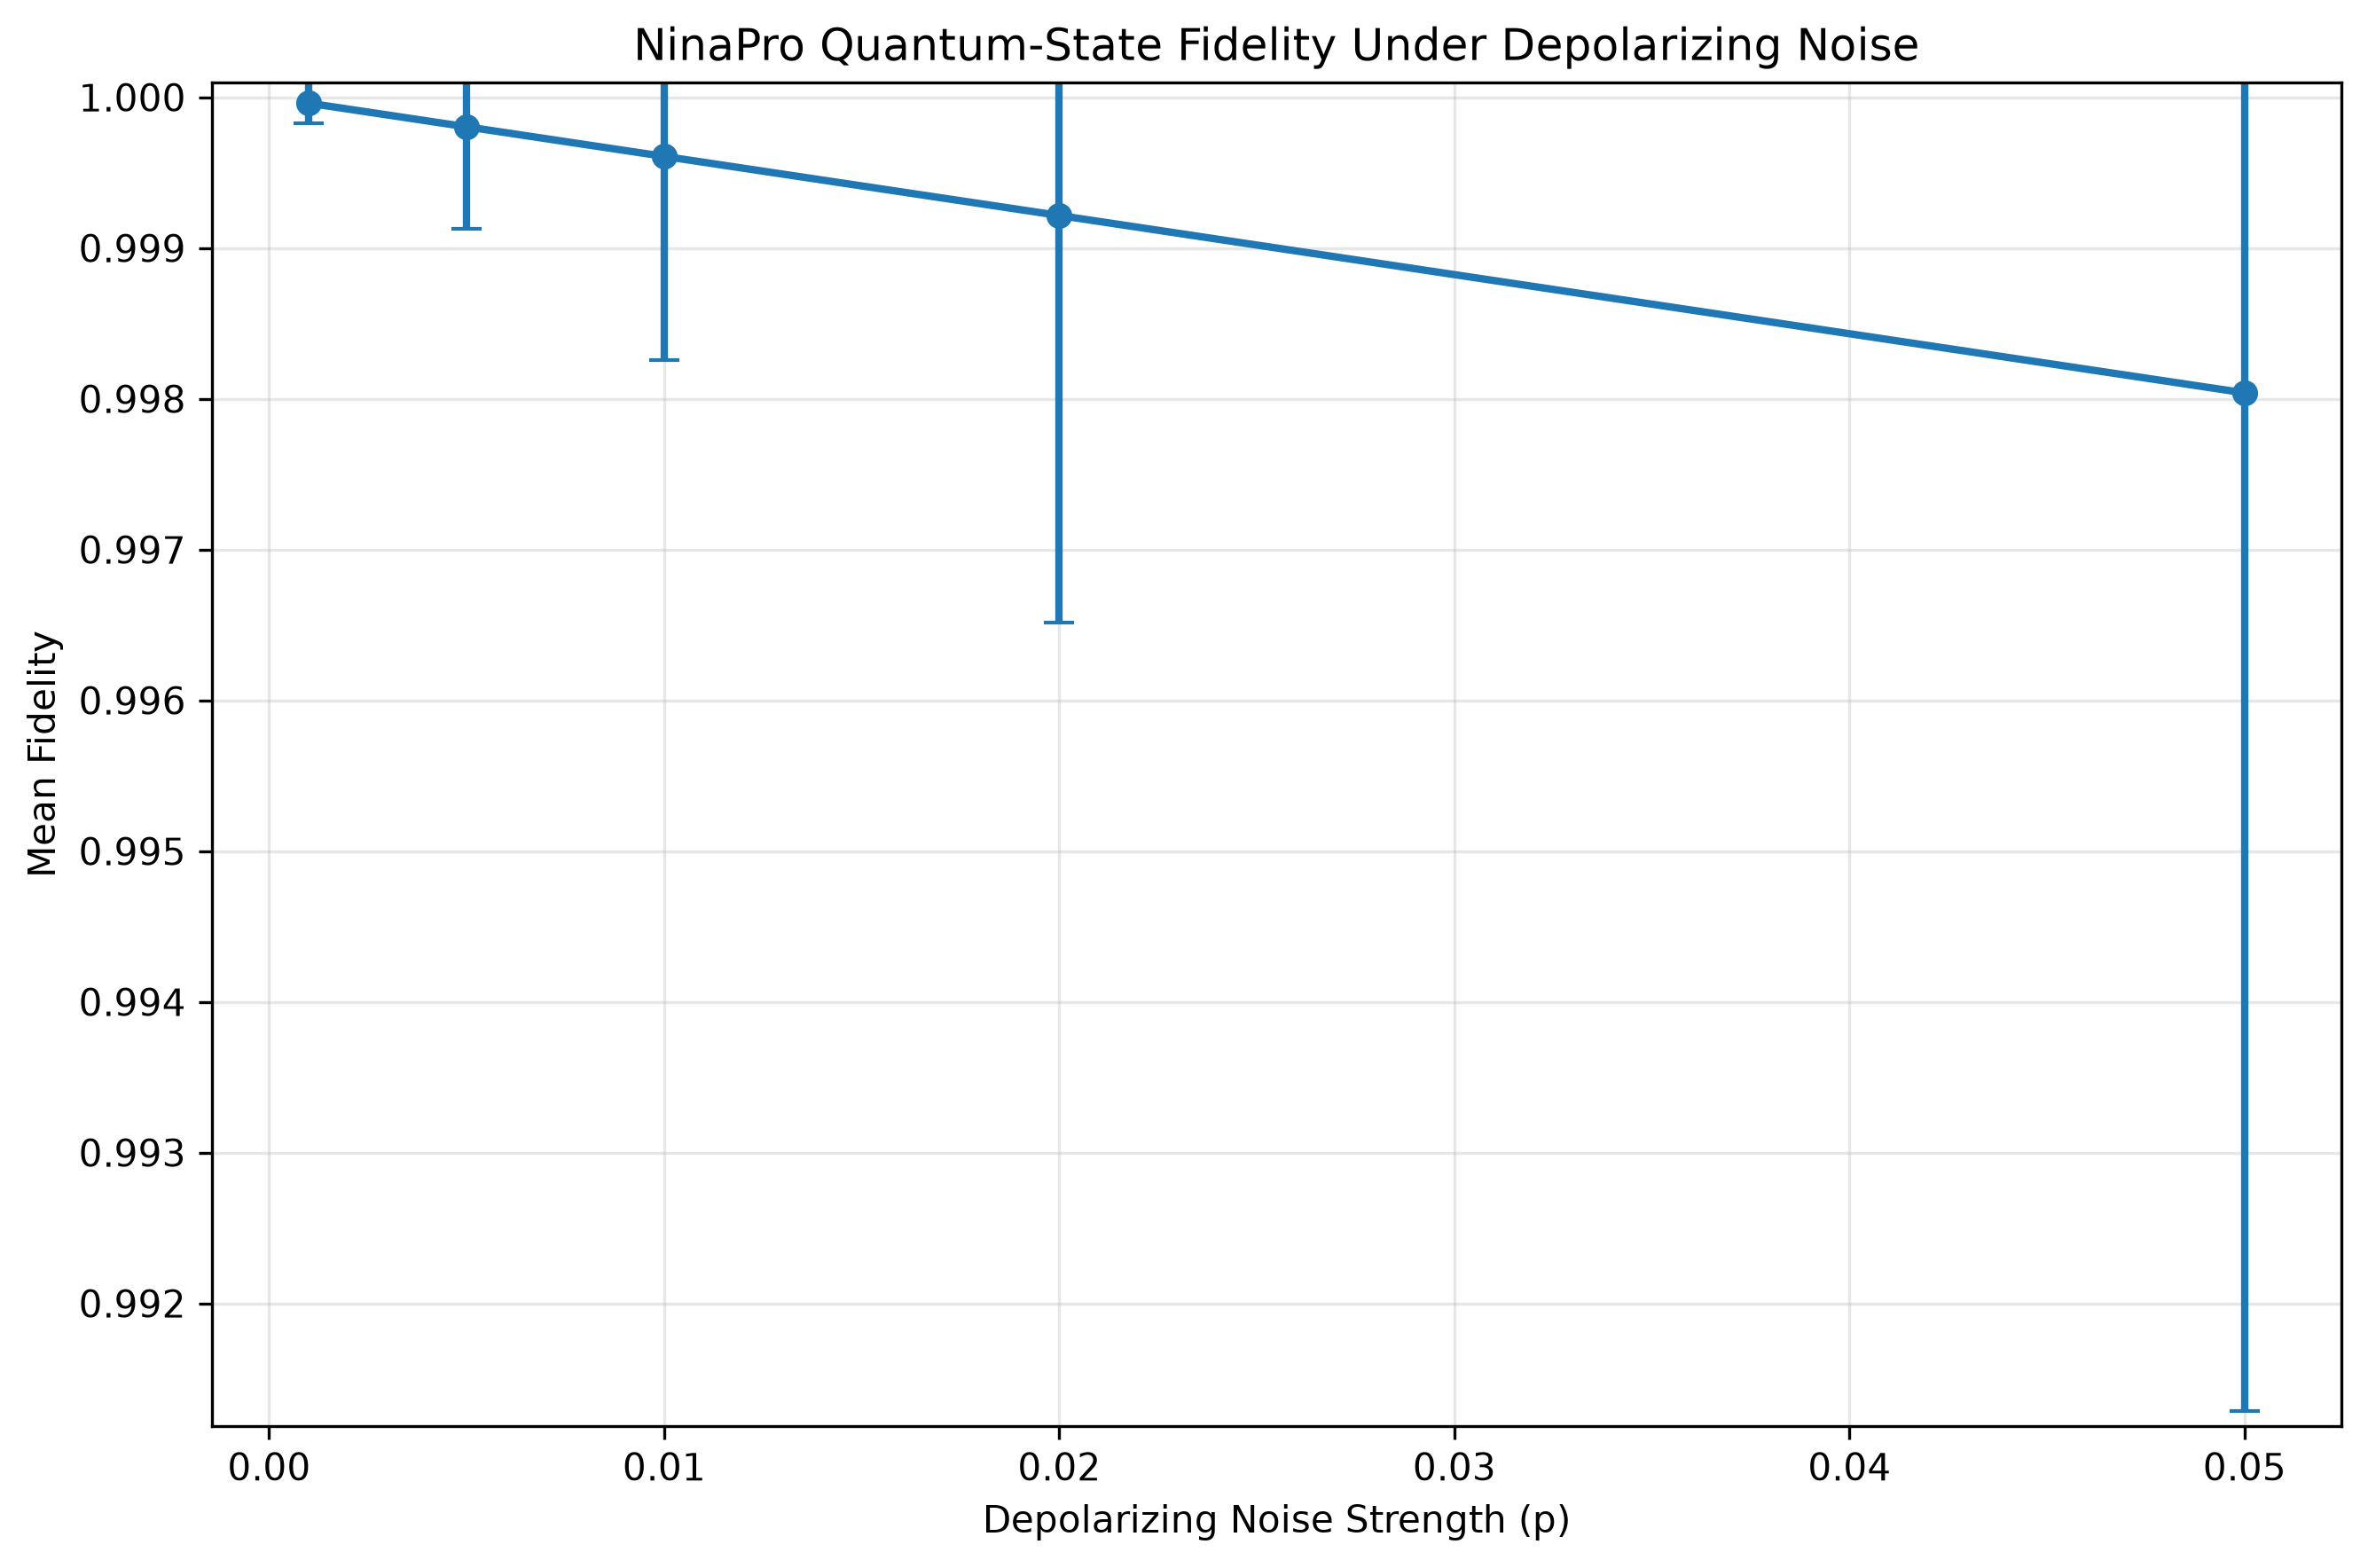
\includegraphics[width=0.90\textwidth]
    {figures/ninapro_noise_fidelity.png}
    \caption{Mean quantum-state fidelity for the 102-sample NinaPro workload
    as depolarizing-noise strength increases. Error bars represent the
    observed fidelity variation across samples.}
    \label{fig:ninapro-noise-fidelity}
\end{figure}

\begin{figure}[H]
    \centering
    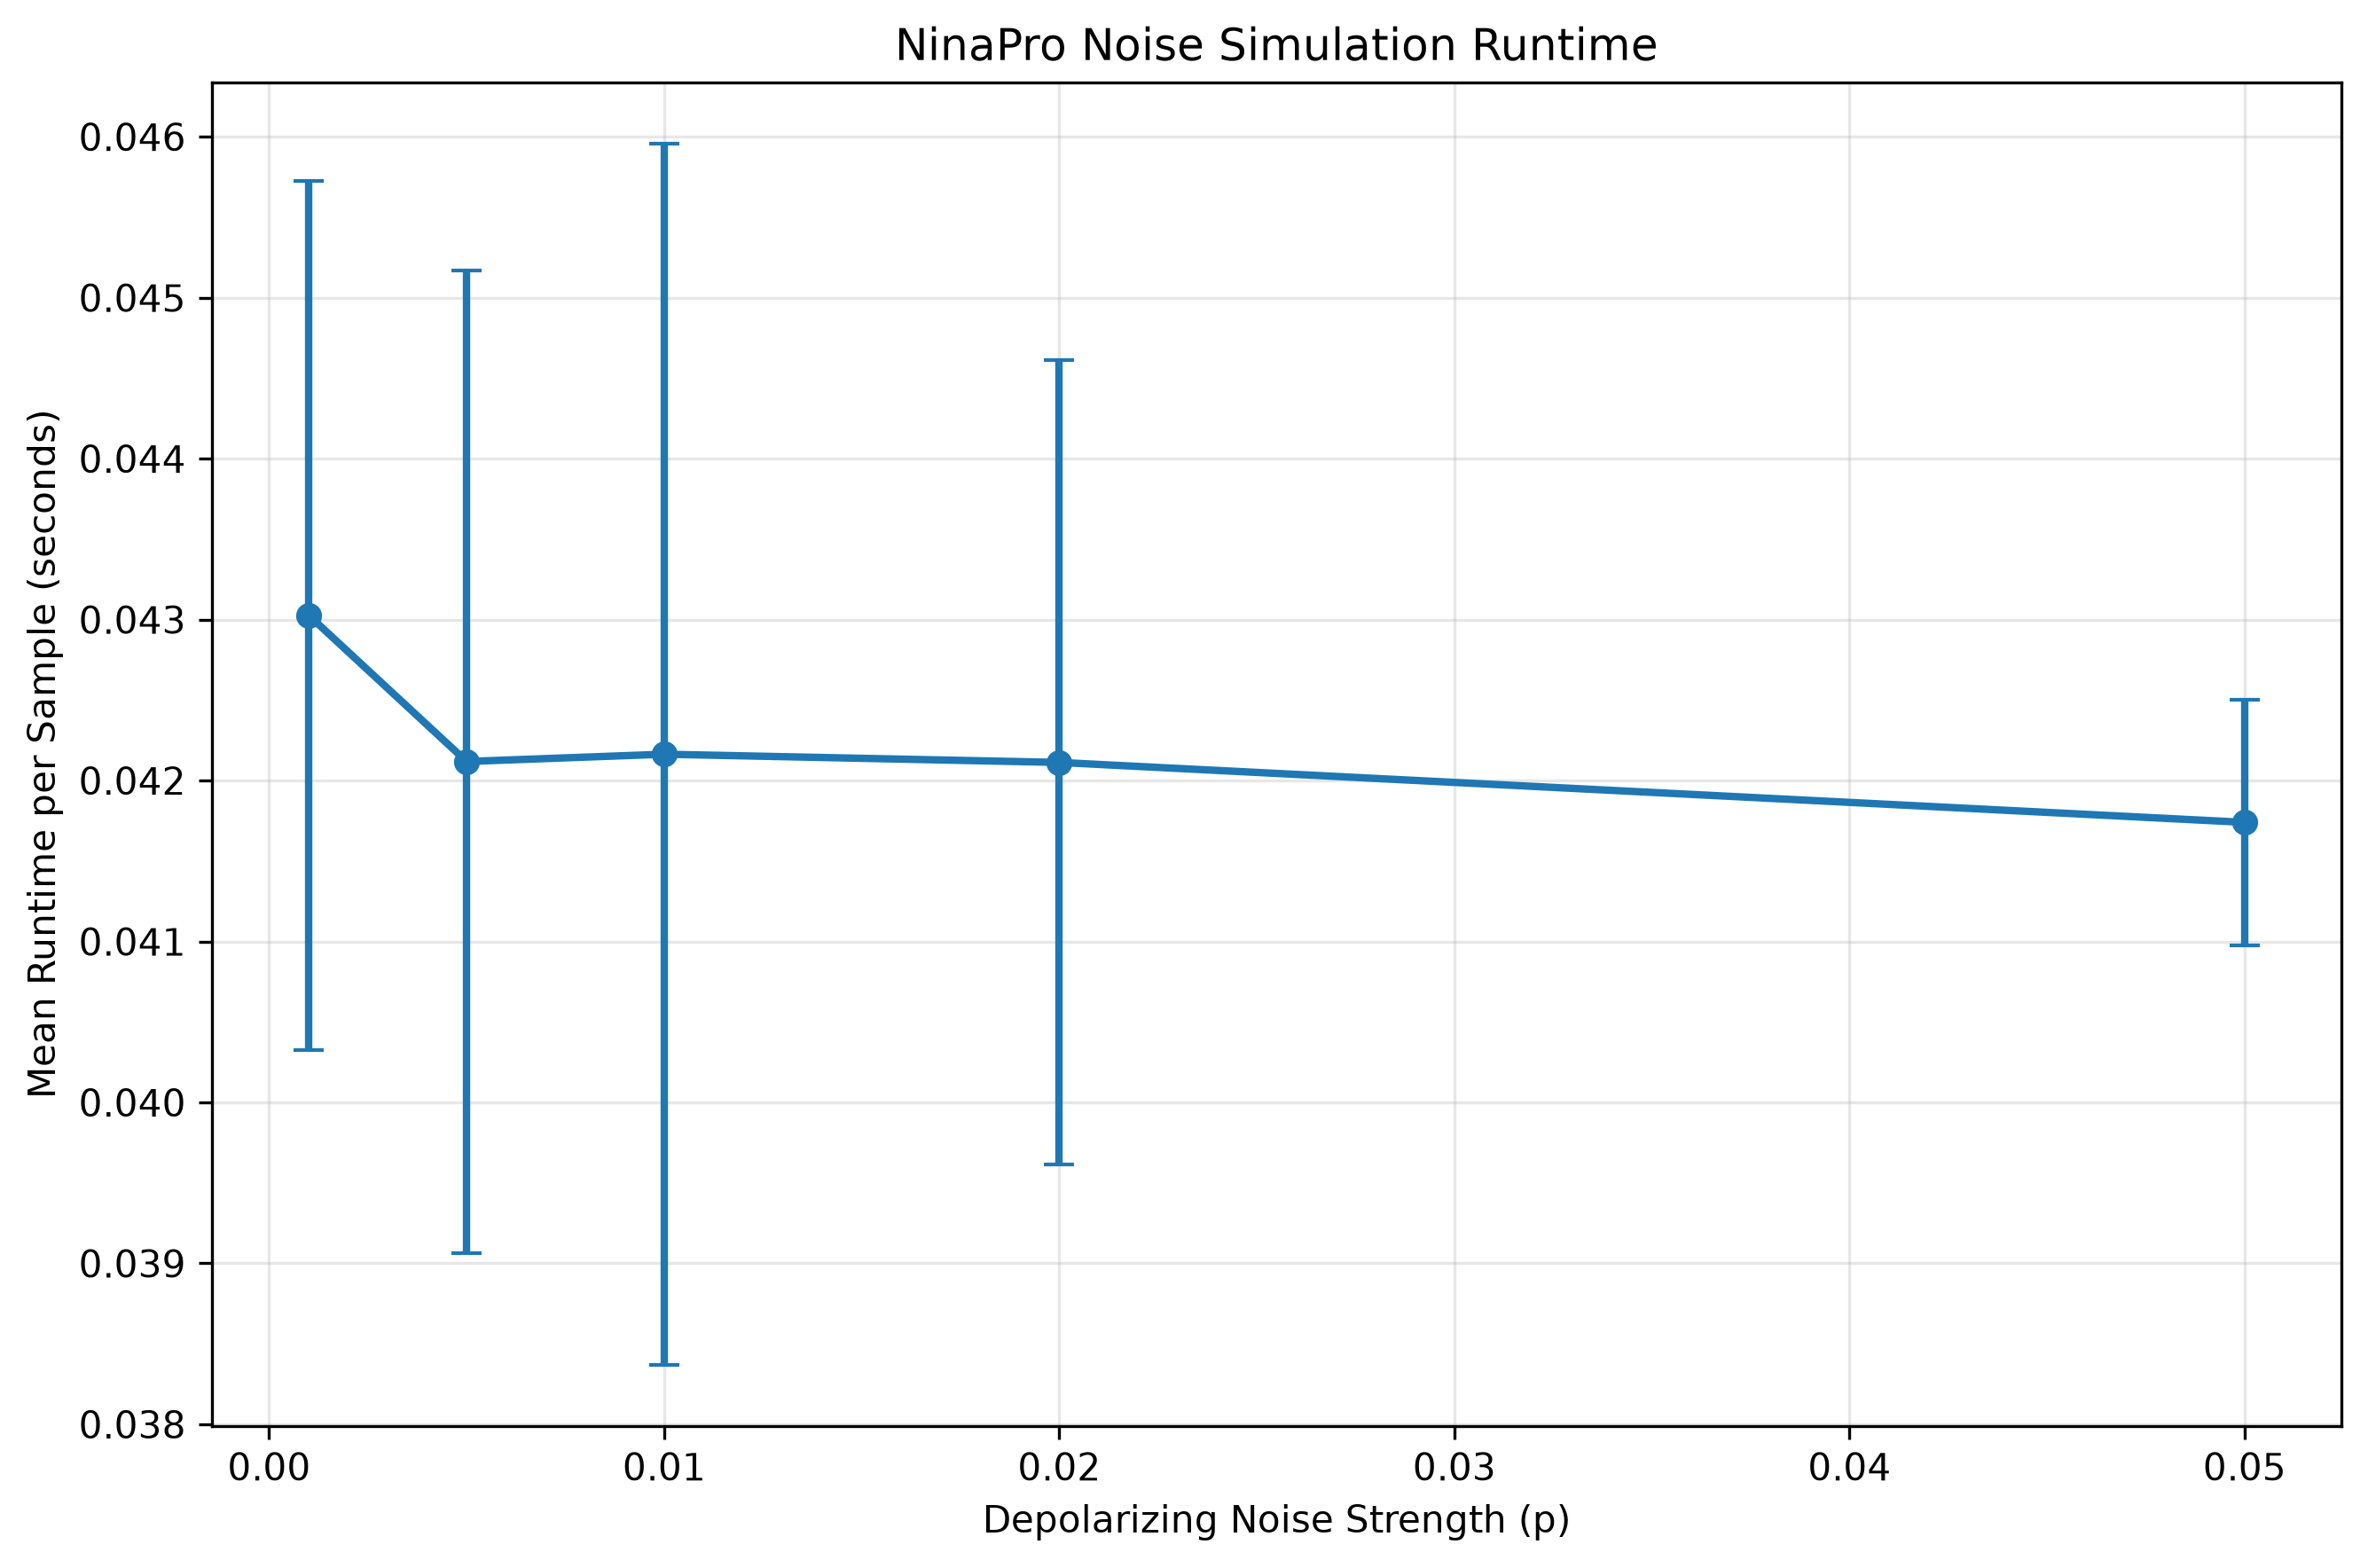
\includegraphics[width=0.90\textwidth]
    {figures/ninapro_noise_runtime.png}
    \caption{Mean simulation runtime per NinaPro sample across the five tested
    depolarizing-noise strengths.}
    \label{fig:ninapro-noise-runtime}
\end{figure}


\subsection{Preliminary Bridges-2 MPI Scaling}
\label{subsec:preliminary-mpi-results}

Before development of the final NinaPro MPI benchmark, an earlier validation
workload was executed on Bridges-2 using 1, 2, and 4 MPI processes. Mean
runtime decreased from approximately 6.1~s with one process to 3.5~s with two
processes and 2.3~s with four processes, corresponding to preliminary speedups
of approximately \(1.74\times\) and \(2.61\times\), respectively.

These measurements established that the SLURM and MPI execution workflow
functioned correctly on Bridges-2. They are retained as preliminary validation
results but are superseded by the final NinaPro scaling experiment reported
below.


\subsection{Final NinaPro MPI Scaling}
\label{subsec:final-mpi-results}

The final distributed-memory benchmark evaluated the NinaPro quantum-kernel
workflow using 1, 2, 4, and 8 MPI processes on Bridges-2. All benchmark
configurations completed successfully, and every timed kernel matrix passed
the numerical validation checks.


\subsubsection{Strong Scaling}

The strong-scaling experiment held the 102-sample, 5253-pair workload constant
while increasing MPI process count. Table~\ref{tab:strong-scaling-results}
summarizes the measured runtime, speedup, and parallel efficiency.

\begin{table}[!htbp]
\centering
\caption{Final NinaPro strong-scaling results on Bridges-2.}
\label{tab:strong-scaling-results}
\begin{tabular}{rrrrr}
\toprule
MPI Processes &
Samples &
Mean Runtime (s) &
Speedup &
Efficiency (\%) \\
\midrule
1 & 102 & 0.168016 & 1.000 & 100.00 \\
2 & 102 & 0.084332 & 1.992 & 99.62 \\
4 & 102 & 0.044457 & 3.779 & 94.48 \\
8 & 102 & 0.024862 & 6.758 & 84.47 \\
\bottomrule
\end{tabular}
\end{table}

Mean runtime decreased from 0.168016~s with one process to 0.084332~s with
two processes, 0.044457~s with four processes, and 0.024862~s with eight
processes. Relative to the single-process baseline, the corresponding measured
speedups were \(1.992\times\), \(3.779\times\), and \(6.758\times\).

Parallel efficiency remained 99.62\% at two processes, 94.48\% at four
processes, and 84.47\% at eight processes. The results therefore show
near-linear scaling at the lower process counts and continued substantial
acceleration through eight MPI processes.

\begin{figure}[H]
    \centering
    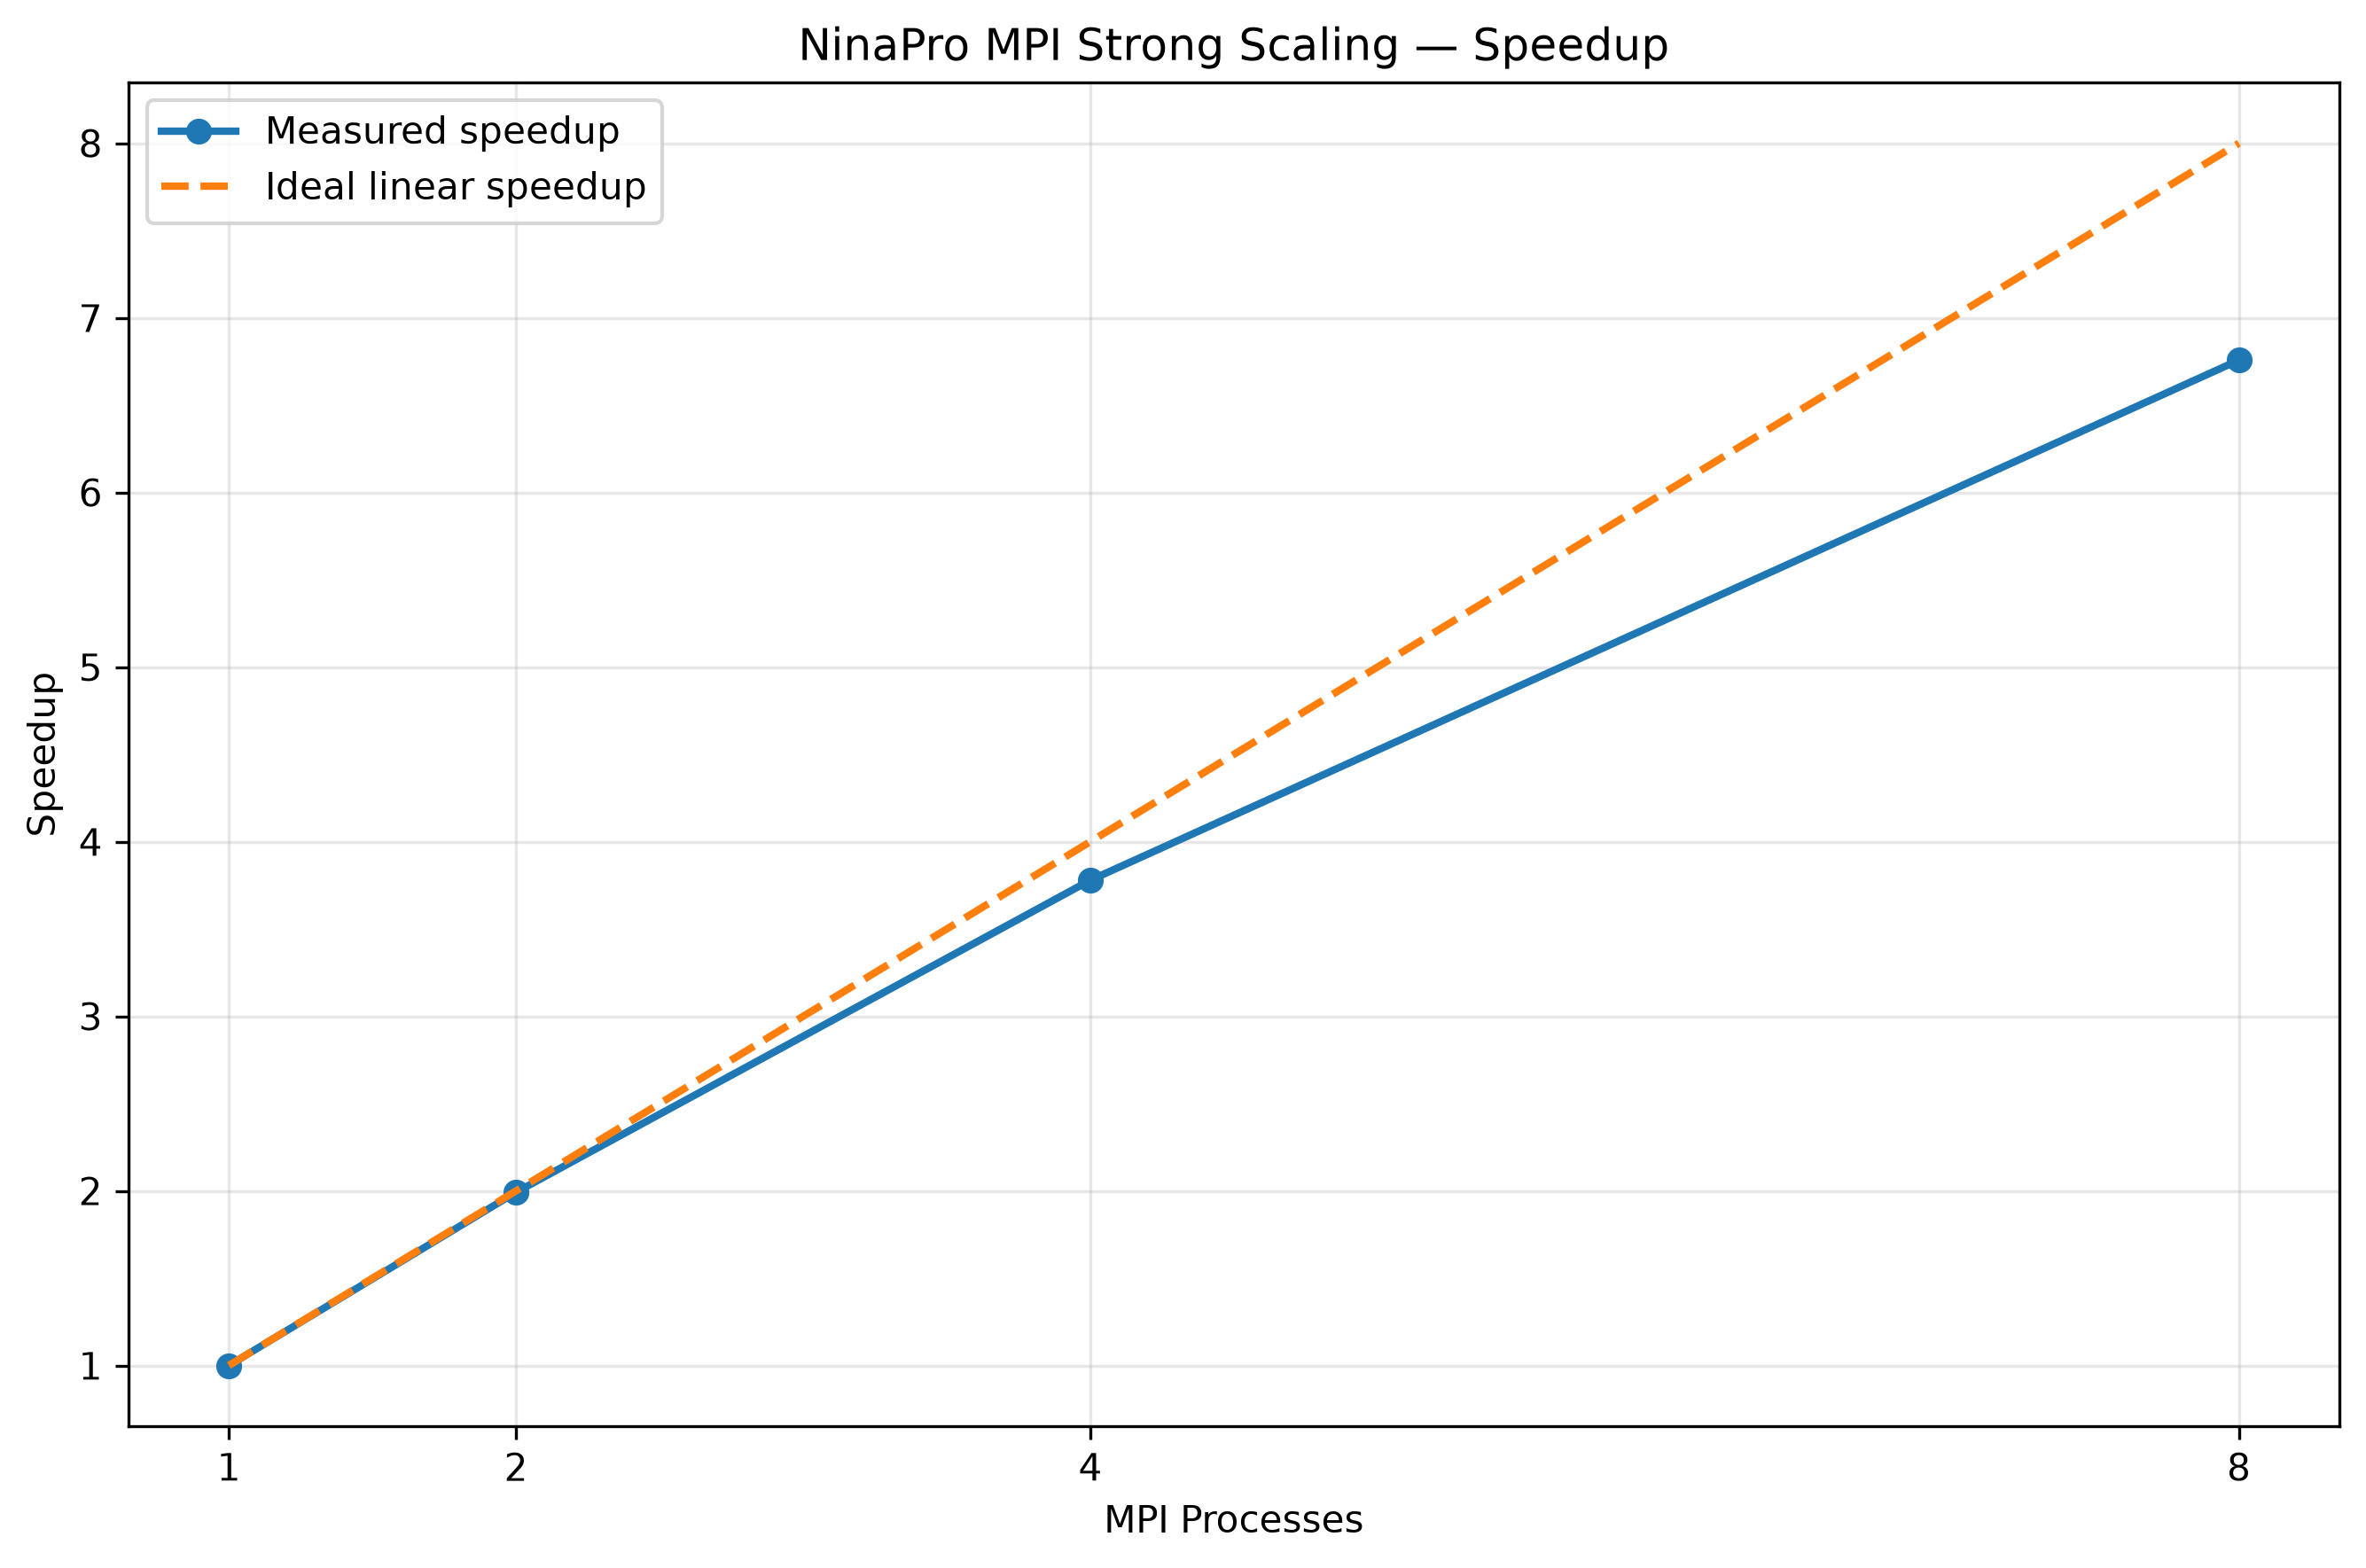
\includegraphics[width=0.90\textwidth]
    {figures/ninapro_mpi_strong_speedup.png}
    \caption{Final NinaPro strong-scaling speedup on Bridges-2 relative to
    the single-process baseline. The dashed line represents ideal linear
    speedup.}
    \label{fig:ninapro-strong-speedup}
\end{figure}


\subsubsection{Weak Scaling}

The weak-scaling experiment increased the number of workload samples with MPI
process count while maintaining approximately 5200 upper-triangular
kernel-pair evaluations per rank.

\begin{table}[!htbp]
\centering
\caption{Final NinaPro kernel-pair weak-scaling results on Bridges-2.}
\label{tab:weak-scaling-results}
\begin{tabular}{rrrrrr}
\toprule
MPI Processes &
Samples &
Kernel Pairs &
Pairs/Rank &
Mean Runtime (s) &
Efficiency (\%) \\
\midrule
1 & 102 & 5253  & 5253.00 & 0.167482 & 100.00 \\
2 & 144 & 10440 & 5220.00 & 0.123327 & 134.95 \\
4 & 204 & 20910 & 5227.50 & 0.094989 & 175.46 \\
8 & 289 & 41905 & 5238.12 & 0.084434 & 197.80 \\
\bottomrule
\end{tabular}
\end{table}

The number of kernel-pair calculations per process remained approximately
constant across the four configurations. Mean runtime nevertheless decreased
from 0.167482~s with one process to 0.123327~s with two processes,
0.094989~s with four processes, and 0.084434~s with eight processes.

The resulting calculated weak-scaling efficiencies exceeded 100\% for the
multi-process configurations. This superlinear result reflects the structure
of the complete timed workflow rather than an increase in computational work
performed by each process. Although kernel-pair evaluations per rank remain
approximately constant, the timed region also includes quantum-state encoding.
Because workload sample count grows approximately with \(\sqrt{P}\), the number
of samples encoded by each rank decreases as process count increases. The
reported weak-scaling efficiency should therefore be interpreted specifically
as kernel-pair weak scaling of the complete implemented workflow.

\begin{figure}[H]
    \centering
    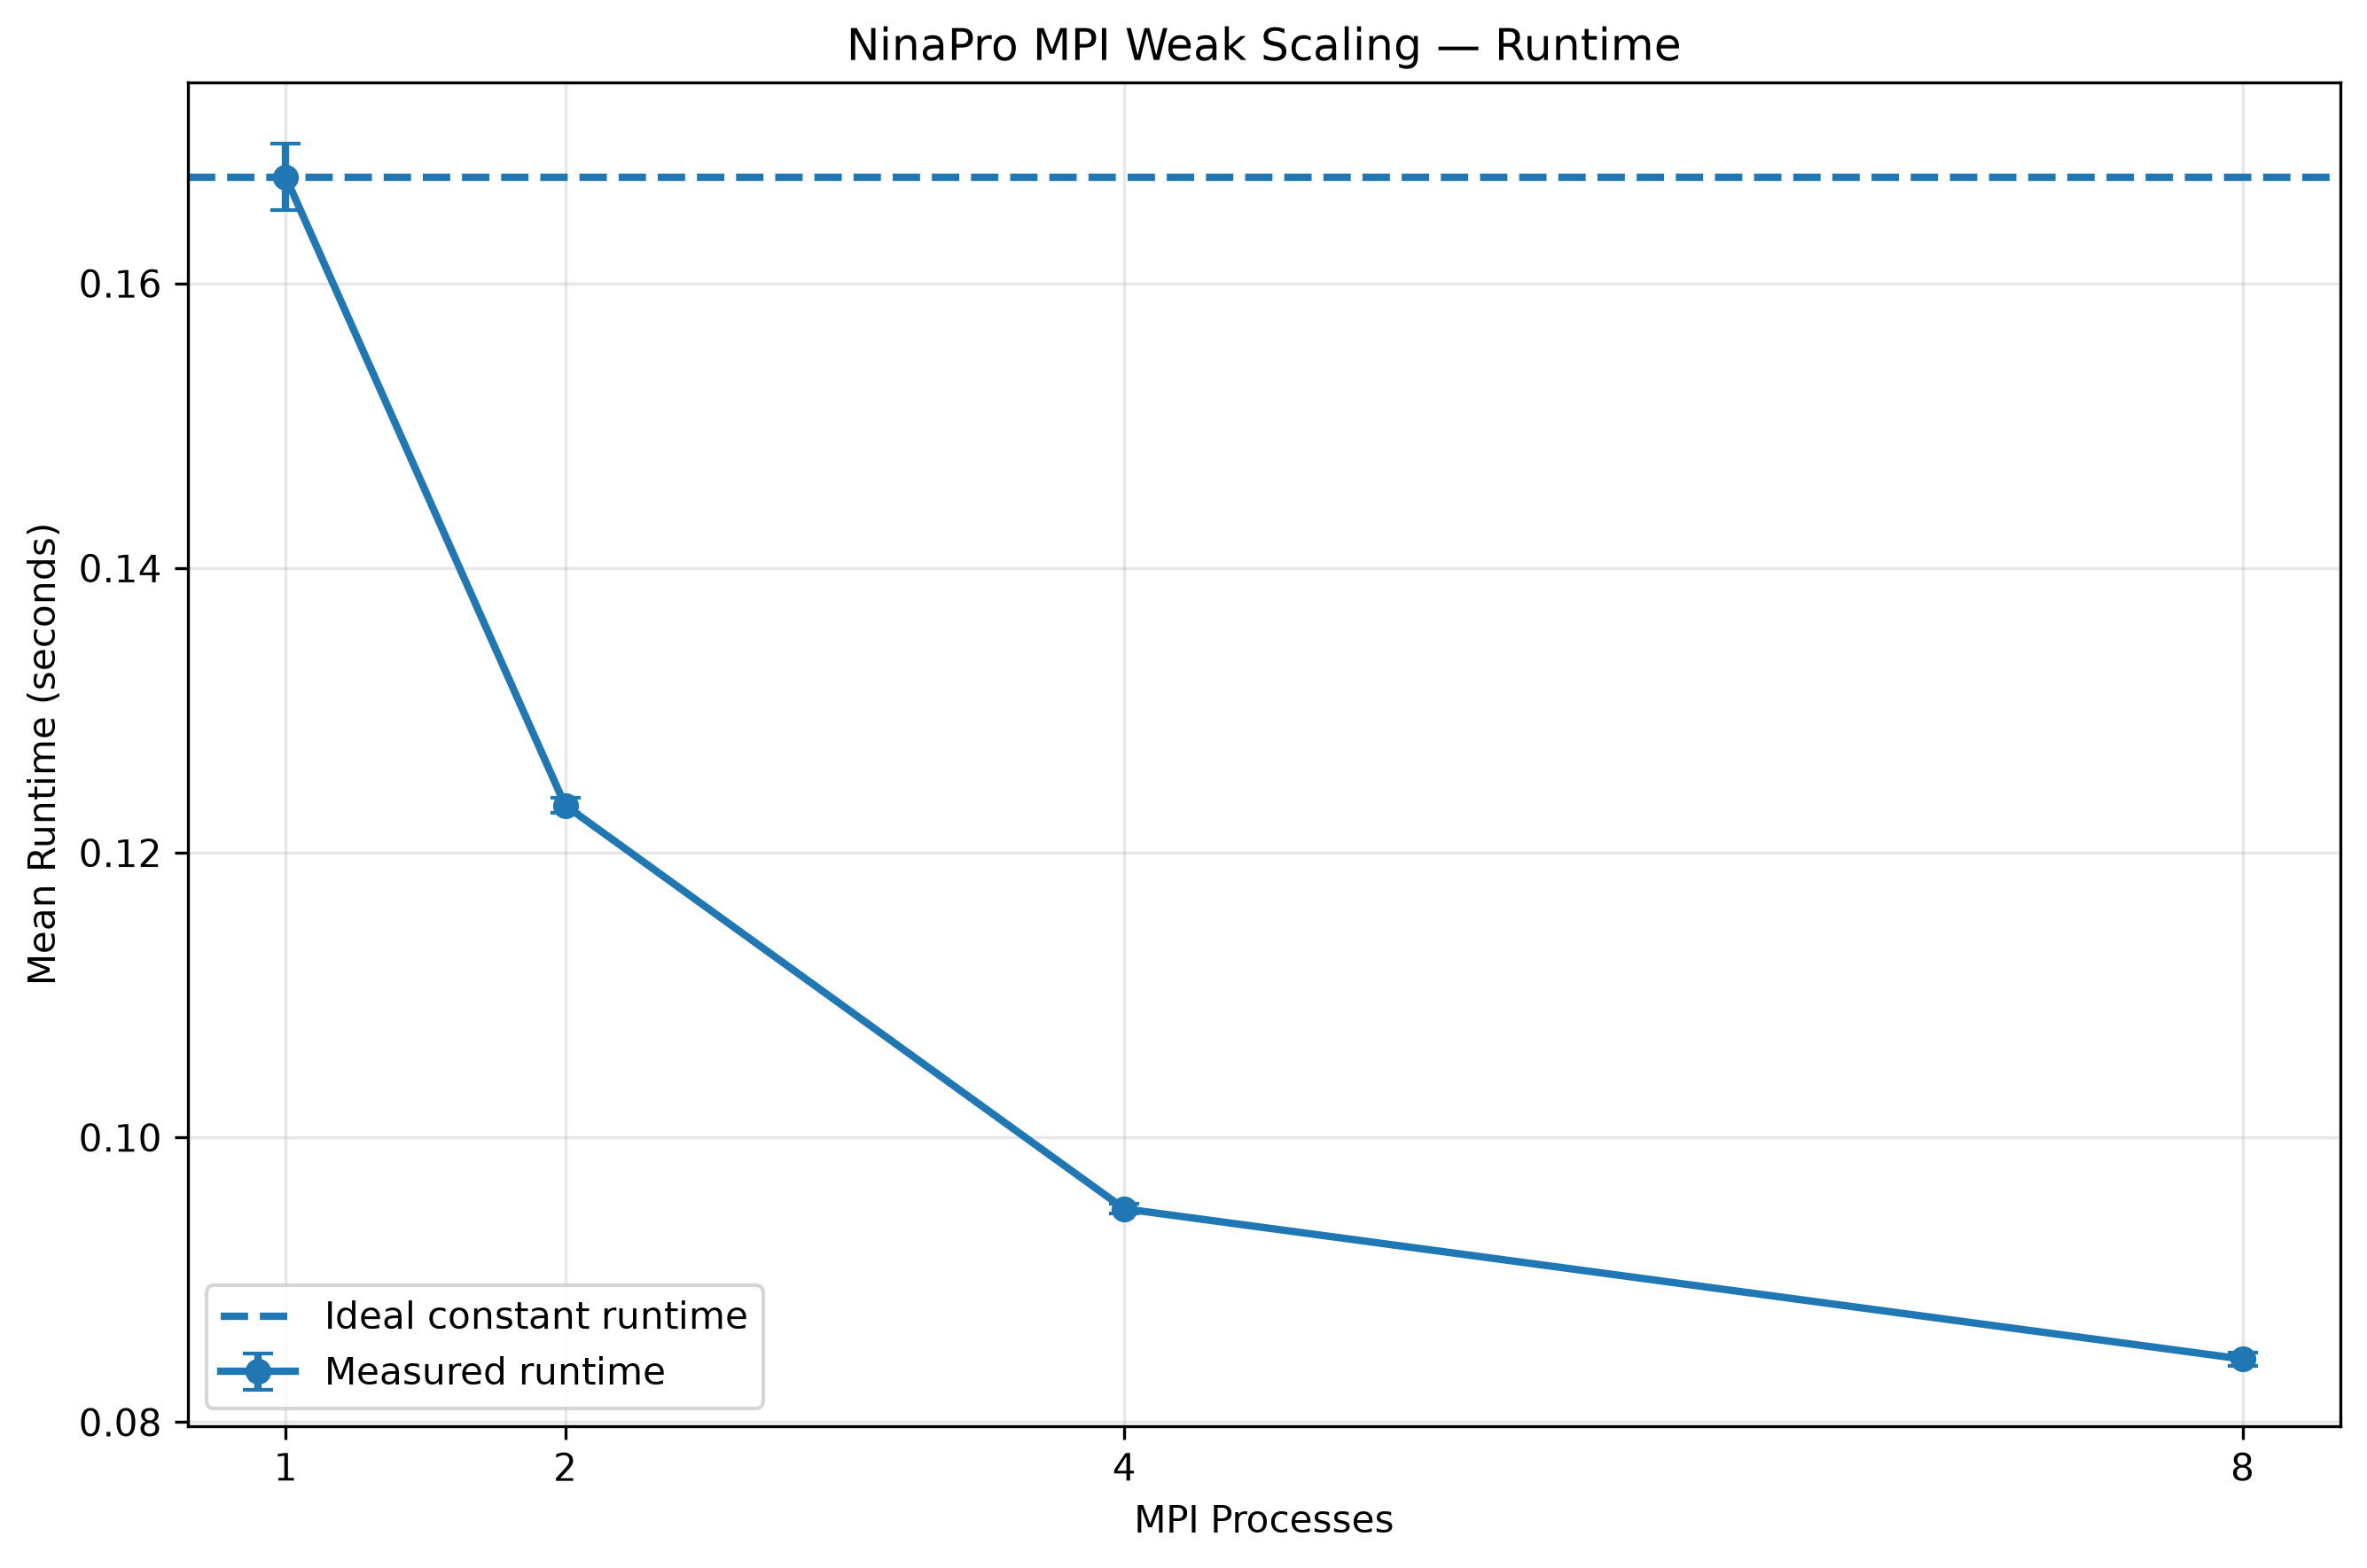
\includegraphics[width=0.90\textwidth]
    {figures/ninapro_mpi_weak_runtime.png}
    \caption{Final NinaPro kernel-pair weak-scaling runtime on Bridges-2.
    The dashed line represents the single-process runtime expected under
    ideal constant-runtime weak scaling.}
    \label{fig:ninapro-weak-runtime}
\end{figure}


\subsubsection{Multi-Node MPI Extension}
\label{subsec:multinode-mpi-results}

The follow-on MPI experiment compared matched MPI process counts using
single-node and multi-node placement. Table~\ref{tab:multinode-mpi-results}
summarizes the resulting runtimes.

\begin{table}[!htbp]
\centering
\caption{Matched single-node and multi-node MPI results for the fixed
102-sample NinaPro quantum-kernel workload on Bridges-2.}
\label{tab:multinode-mpi-results}

\setlength{\tabcolsep}{4pt}

\begin{tabular}{rrrrr}
\toprule
MPI Ranks &
Nodes &
Ranks/Node &
Mean Runtime (s) &
Std. (s) \\
\midrule
8  & 1 & 8  & 0.025199 & 0.001515 \\
8  & 2 & 4  & 0.026109 & 0.000258 \\
16 & 1 & 16 & 0.014399 & 0.000372 \\
16 & 2 & 8  & 0.020099 & 0.001448 \\
32 & 1 & 32 & 0.009882 & 0.000359 \\
32 & 4 & 8  & 0.014152 & 0.000246 \\
\bottomrule
\end{tabular}
\end{table}

At eight MPI processes, distributing the ranks across two nodes produced a
mean runtime of 0.026109~s compared with 0.025199~s when all eight ranks were
placed on one node. This represents a modest runtime increase of approximately
3.61\%.

The effect of inter-node placement became substantially larger at the higher
process counts. At sixteen MPI processes, the single-node configuration
completed in 0.014399~s, whereas the two-node configuration required
0.020099~s, an increase of approximately 39.59\%. At thirty-two processes,
the single-node configuration completed in 0.009882~s compared with
0.014152~s when the same number of processes was distributed across four
nodes, corresponding to approximately 43.21\% higher runtime.

\begin{figure}[H]
    \centering
    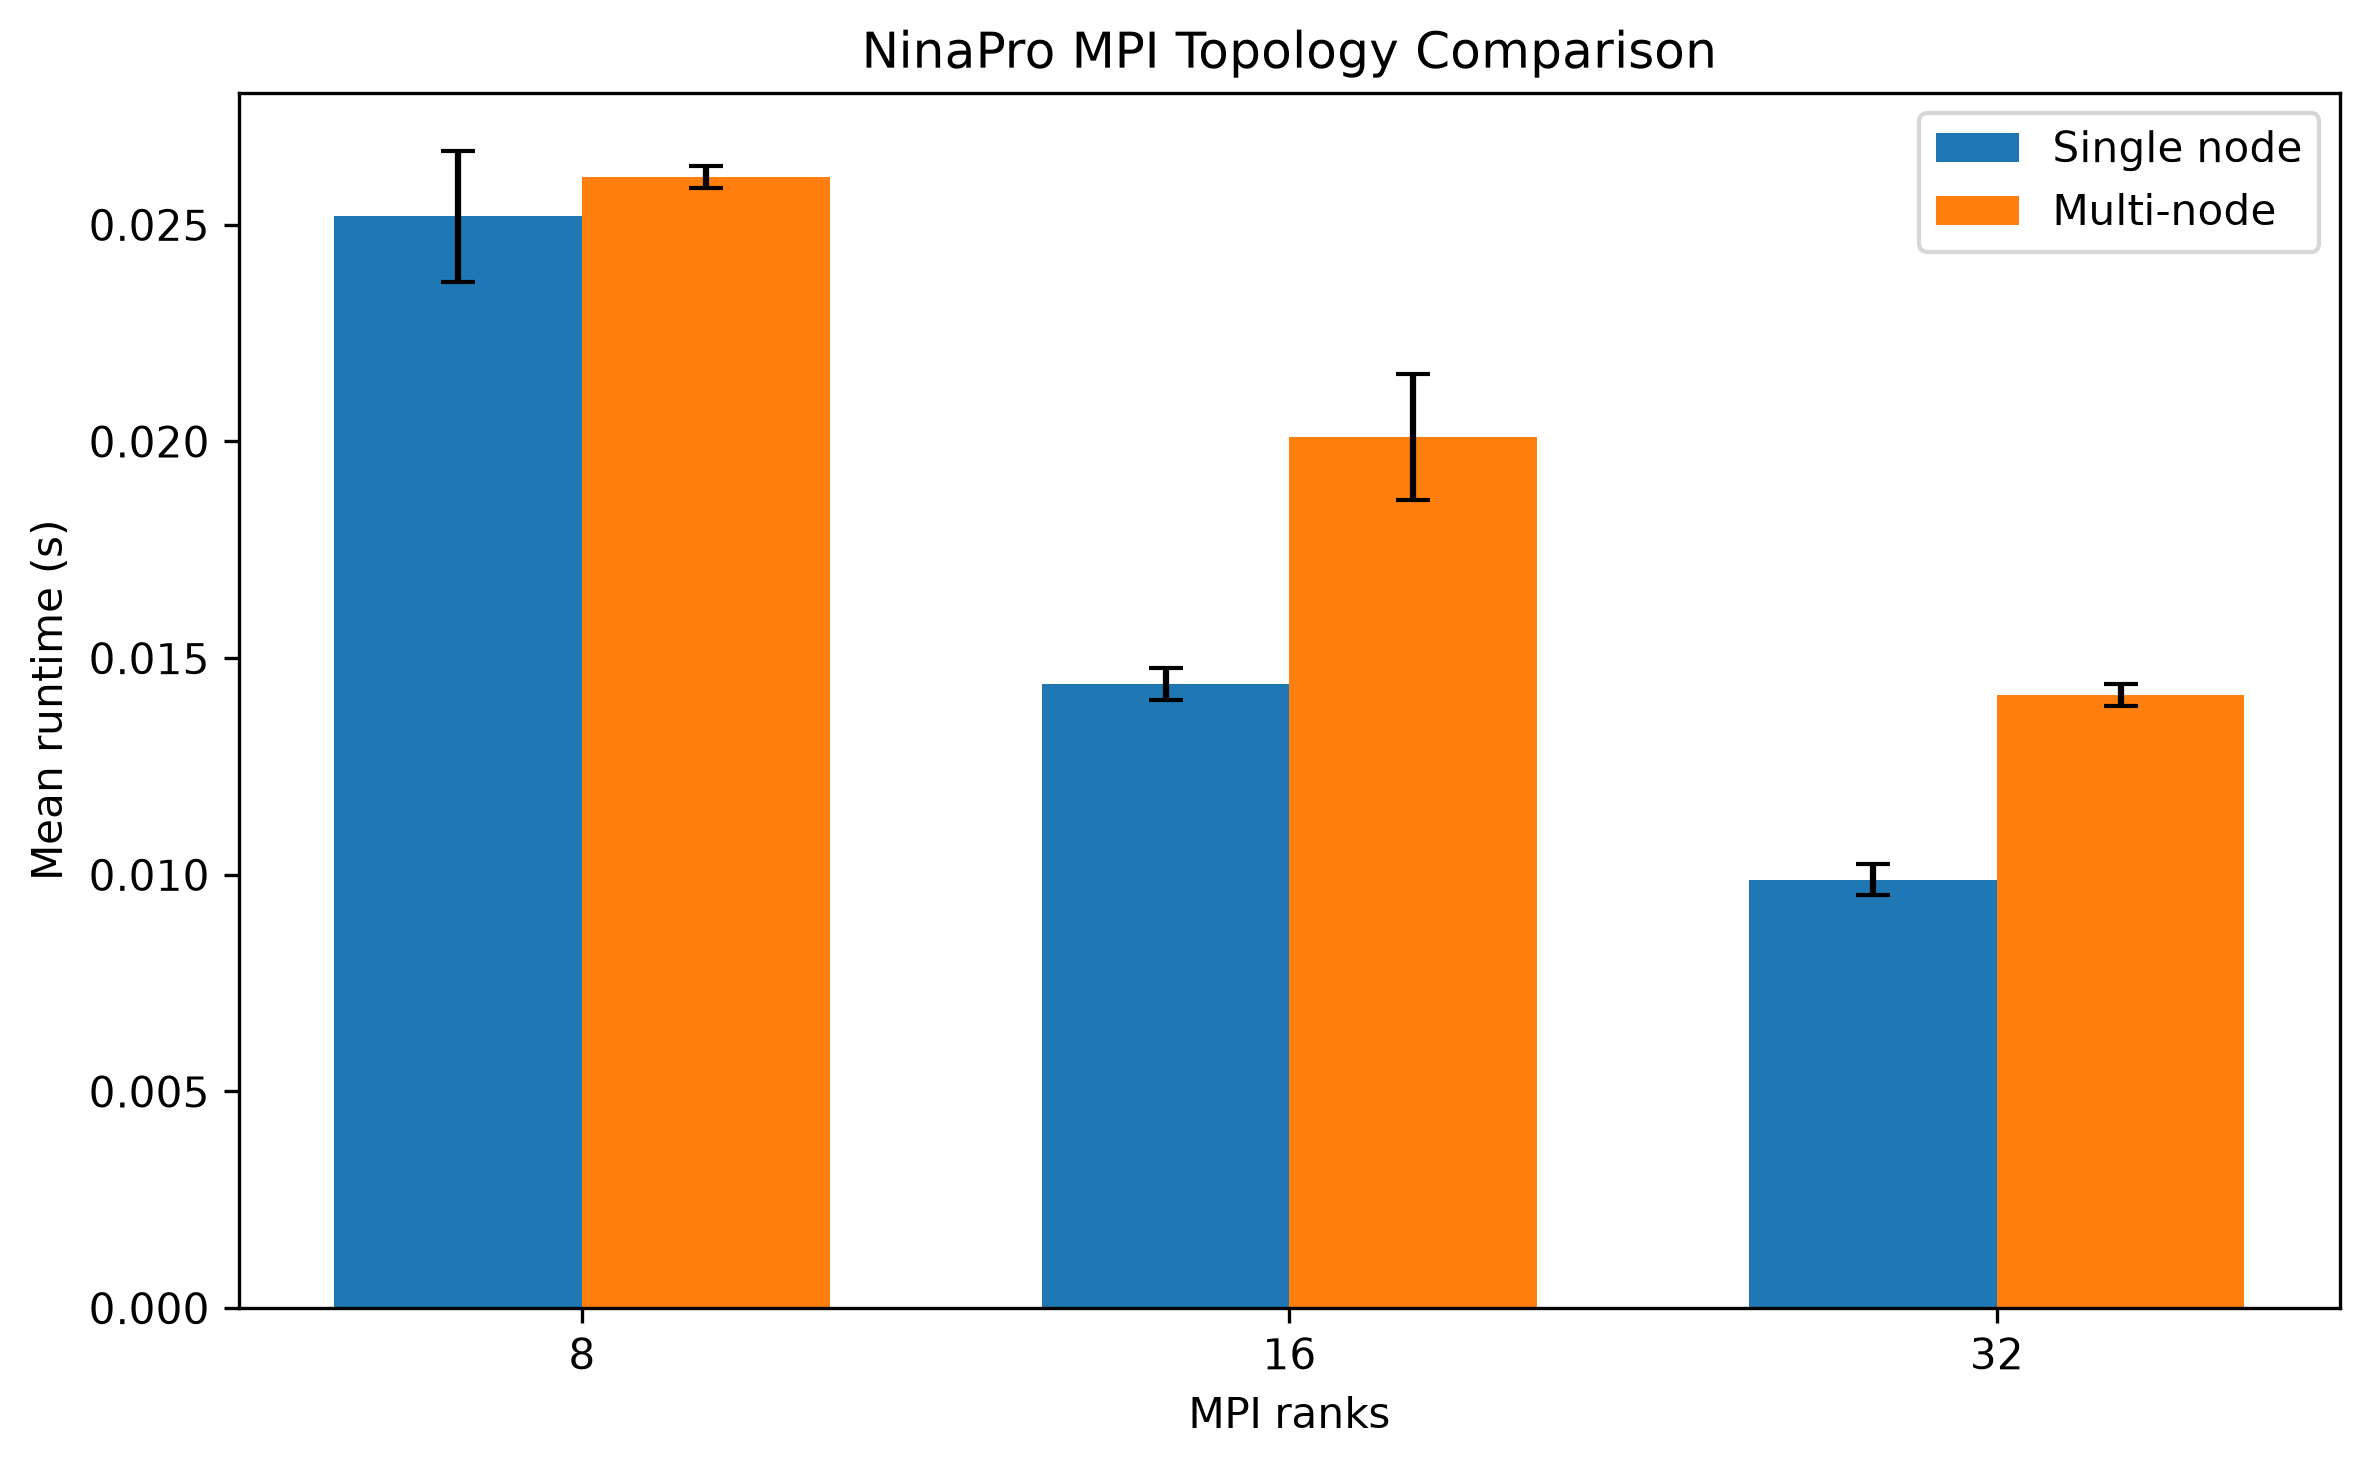
\includegraphics[width=0.90\textwidth]
    {figures/ninapro_mpi_multinode_runtime.png}
    \caption{Matched-rank MPI topology comparison for the fixed 102-sample
    NinaPro quantum-kernel workload on Bridges-2. Single-node configurations
    place all MPI ranks on one Regular Memory node. The multi-node
    configurations use two nodes for the 8- and 16-rank tests and four nodes
    for the 32-rank test. Error bars represent the standard deviation across
    five timed iterations.}
    \label{fig:ninapro-multinode-runtime}
\end{figure}

Despite the inter-node overhead, increasing the total MPI process count
continued to reduce runtime. Within the single-node configurations, increasing
from 8 to 16 processes produced approximately a \(1.75\times\) speedup, while
increasing from 16 to 32 processes produced an additional
\(1.46\times\) speedup. Relative to the eight-process single-node
configuration, thirty-two processes on one node reduced runtime by
approximately \(2.55\times\).

The multi-node configurations also benefited from increasing process count,
but less efficiently. Runtime decreased from 0.026109~s at eight processes
across two nodes to 0.020099~s at sixteen processes across two nodes and
0.014152~s at thirty-two processes across four nodes. These measurements show
that additional MPI parallelism continued to improve performance, while
inter-node communication reduced the benefit obtained from the additional
processes.

\subsubsection{Large Real-Data Multi-Node MPI Scaling}
\label{subsec:realdata-multinode-results}

To evaluate multi-node MPI behavior under a substantially larger real-data
workload, the NinaPro dataset was expanded from one to seven distinct
non-overlapping 512-sample EMG windows per gesture/repetition segment. With
17 gestures and 6 repetitions, this produced 714 distinct real EMG windows
and 255,255 upper-triangular quantum-kernel pairs.

Table~\ref{tab:realdata-multinode-results} summarizes the measured results.
Unlike the smaller 102-sample workload, matched single-node and multi-node
configurations produced nearly identical runtimes.

\begin{table}[!htbp]
\centering
\caption{Large real-data MPI scaling results using 714 distinct NinaPro EMG
windows and 255,255 quantum-kernel pairs on Bridges-2.}
\label{tab:realdata-multinode-results}

\setlength{\tabcolsep}{4pt}

\begin{tabular}{rrrrrr}
\toprule
MPI Ranks &
Nodes &
Ranks/Node &
Mean Runtime (s) &
Speedup &
Efficiency (\%) \\
\midrule
1  & 1 & 1  & 1.623986 & 1.000  & 100.00 \\
8  & 1 & 8  & 0.281209 & 5.775  & 72.19 \\
8  & 2 & 4  & 0.282289 & 5.753  & 71.91 \\
16 & 1 & 16 & 0.187434 & 8.664  & 54.15 \\
16 & 2 & 8  & 0.187977 & 8.639  & 54.00 \\
32 & 1 & 32 & 0.136789 & 11.872 & 37.10 \\
32 & 4 & 8  & 0.136360 & 11.910 & 37.22 \\
\bottomrule
\end{tabular}
\end{table}

At eight MPI processes, distributing the workload across two nodes changed
mean runtime from 0.281209~s to 0.282289~s, a difference of approximately
0.38\%. At sixteen processes, runtime changed from 0.187434~s on one node
to 0.187977~s across two nodes, a difference of approximately 0.29\%.
At thirty-two processes, the four-node configuration completed in
0.136360~s compared with 0.136789~s on one node. This difference was only
approximately 0.31\% and was smaller than the observed run-to-run variation.

These results indicate that the inter-node communication overhead observed
for the smaller workload was largely amortized when the number of real
kernel-pair evaluations increased. The larger workload therefore scaled
similarly whether a fixed number of MPI ranks was placed on one node or
distributed across multiple Bridges-2 nodes.


\subsubsection{Full-Capacity Real-Data MPI Scaling}
\label{subsec:fullcapacity-mpi-results}

A final MPI experiment used every complete non-overlapping 512-sample window
available from the selected NinaPro recording. Across the 102
gesture--repetition segments, this produced 1,404 distinct real EMG windows
and 986,310 upper-triangular quantum-kernel pair evaluations.

The first part of the experiment evaluated process-count scaling on a single
Bridges-2 Regular Memory node using 1, 8, 16, 32, 64, and 128 MPI ranks. The
second part held the total process count fixed at 128 ranks while distributing
those processes across 1, 2, 4, 8, and 16 physical nodes.

\begin{table}[!htbp]
\centering
\caption{Full-capacity NinaPro MPI scaling using 1,404 distinct real EMG
windows and 986,310 quantum-kernel pairs on Bridges-2.}
\label{tab:fullcapacity-mpi}

\setlength{\tabcolsep}{4pt}

\begin{tabular}{rrrrrr}
\toprule
MPI Ranks &
Nodes &
Ranks/Node &
Mean Runtime (s) &
Speedup &
Efficiency (\%) \\
\midrule
1   & 1  & 1   & 4.198034 & 1.000  & 100.00 \\
8   & 1  & 8   & 0.818761 & 5.127  & 64.09 \\
16  & 1  & 16  & 0.565091 & 7.429  & 46.43 \\
32  & 1  & 32  & 0.448628 & 9.357  & 29.24 \\
64  & 1  & 64  & 0.437852 & 9.588  & 14.98 \\
128 & 1  & 128 & 0.378437 & 11.093 & 8.67 \\
128 & 2  & 64  & 0.389714 & 10.772 & 8.42 \\
128 & 4  & 32  & 0.369076 & 11.374 & 8.89 \\
128 & 8  & 16  & 0.367011 & 11.438 & 8.94 \\
128 & 16 & 8   & 0.365481 & 11.486 & 8.97 \\
\bottomrule
\end{tabular}
\end{table}

\begin{figure}[H]
    \centering
    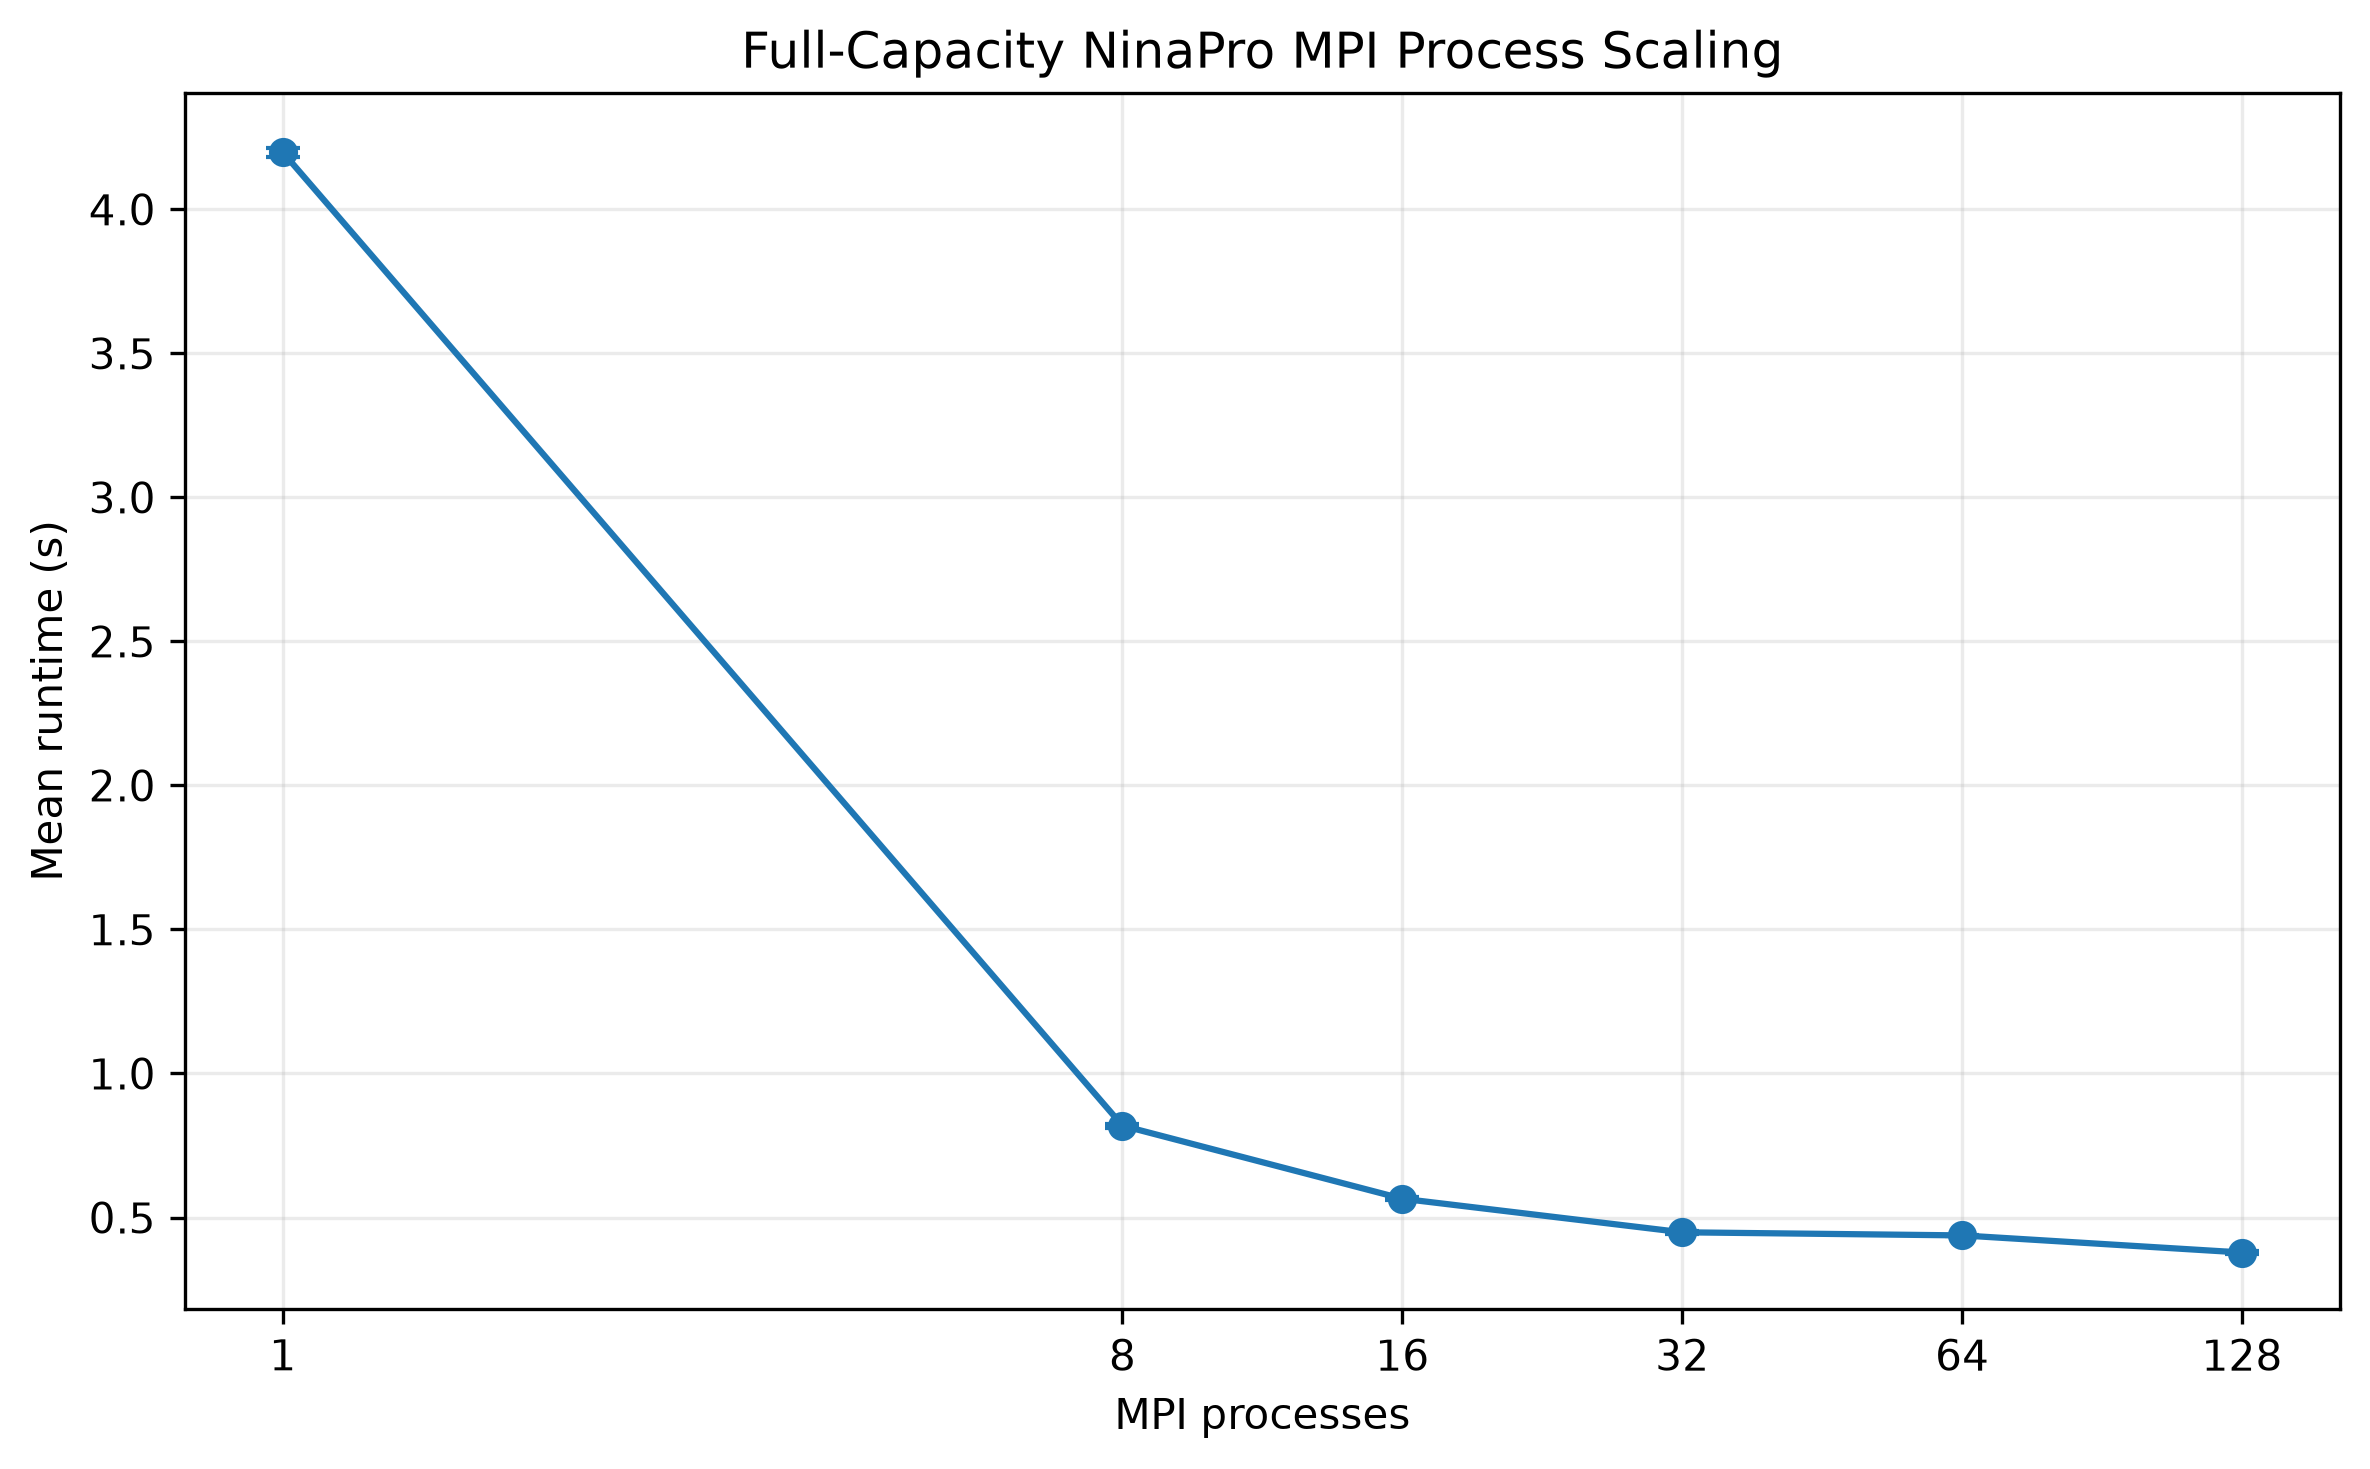
\includegraphics[width=0.90\textwidth]
    {figures/ninapro_fullcapacity_process_scaling.png}
    \caption{Single-node process scaling for the full-capacity NinaPro
    workload containing 1,404 distinct real EMG windows and 986,310
    quantum-kernel pairs. Error bars represent the standard deviation
    across five timed runs.}
    \label{fig:fullcapacity-process-scaling}
\end{figure}

For the single-node process-scaling experiment, mean runtime decreased from
4.198034~s with one MPI process to 0.818761~s with eight processes,
0.565091~s with sixteen processes, 0.448628~s with thirty-two processes,
0.437852~s with sixty-four processes, and 0.378437~s with 128 processes.
Relative to the single-process baseline, the 128-process single-node
configuration achieved an \(11.093\times\) speedup.

Parallel efficiency decreased as process count increased, from 64.09\% at
eight processes to 46.43\% at sixteen, 29.24\% at thirty-two, 14.98\% at
sixty-four, and 8.67\% at 128 processes. The runtime reduction therefore
continued through 128 processes, but with substantial diminishing returns.

Holding the total process count fixed at 128 provided a direct comparison of
physical-node placement. Mean runtime was 0.378437~s on one node,
0.389714~s on two nodes, 0.369076~s on four nodes, 0.367011~s on eight
nodes, and 0.365481~s on sixteen nodes.

The fastest measured configuration used 128 MPI processes distributed across
16 physical nodes, with eight ranks assigned to each node. This configuration
achieved an \(11.486\times\) speedup relative to the one-process baseline.
Compared with the 128-process single-node configuration, the sixteen-node
configuration reduced mean runtime by approximately 3.42\%.

\begin{figure}[H]
    \centering
    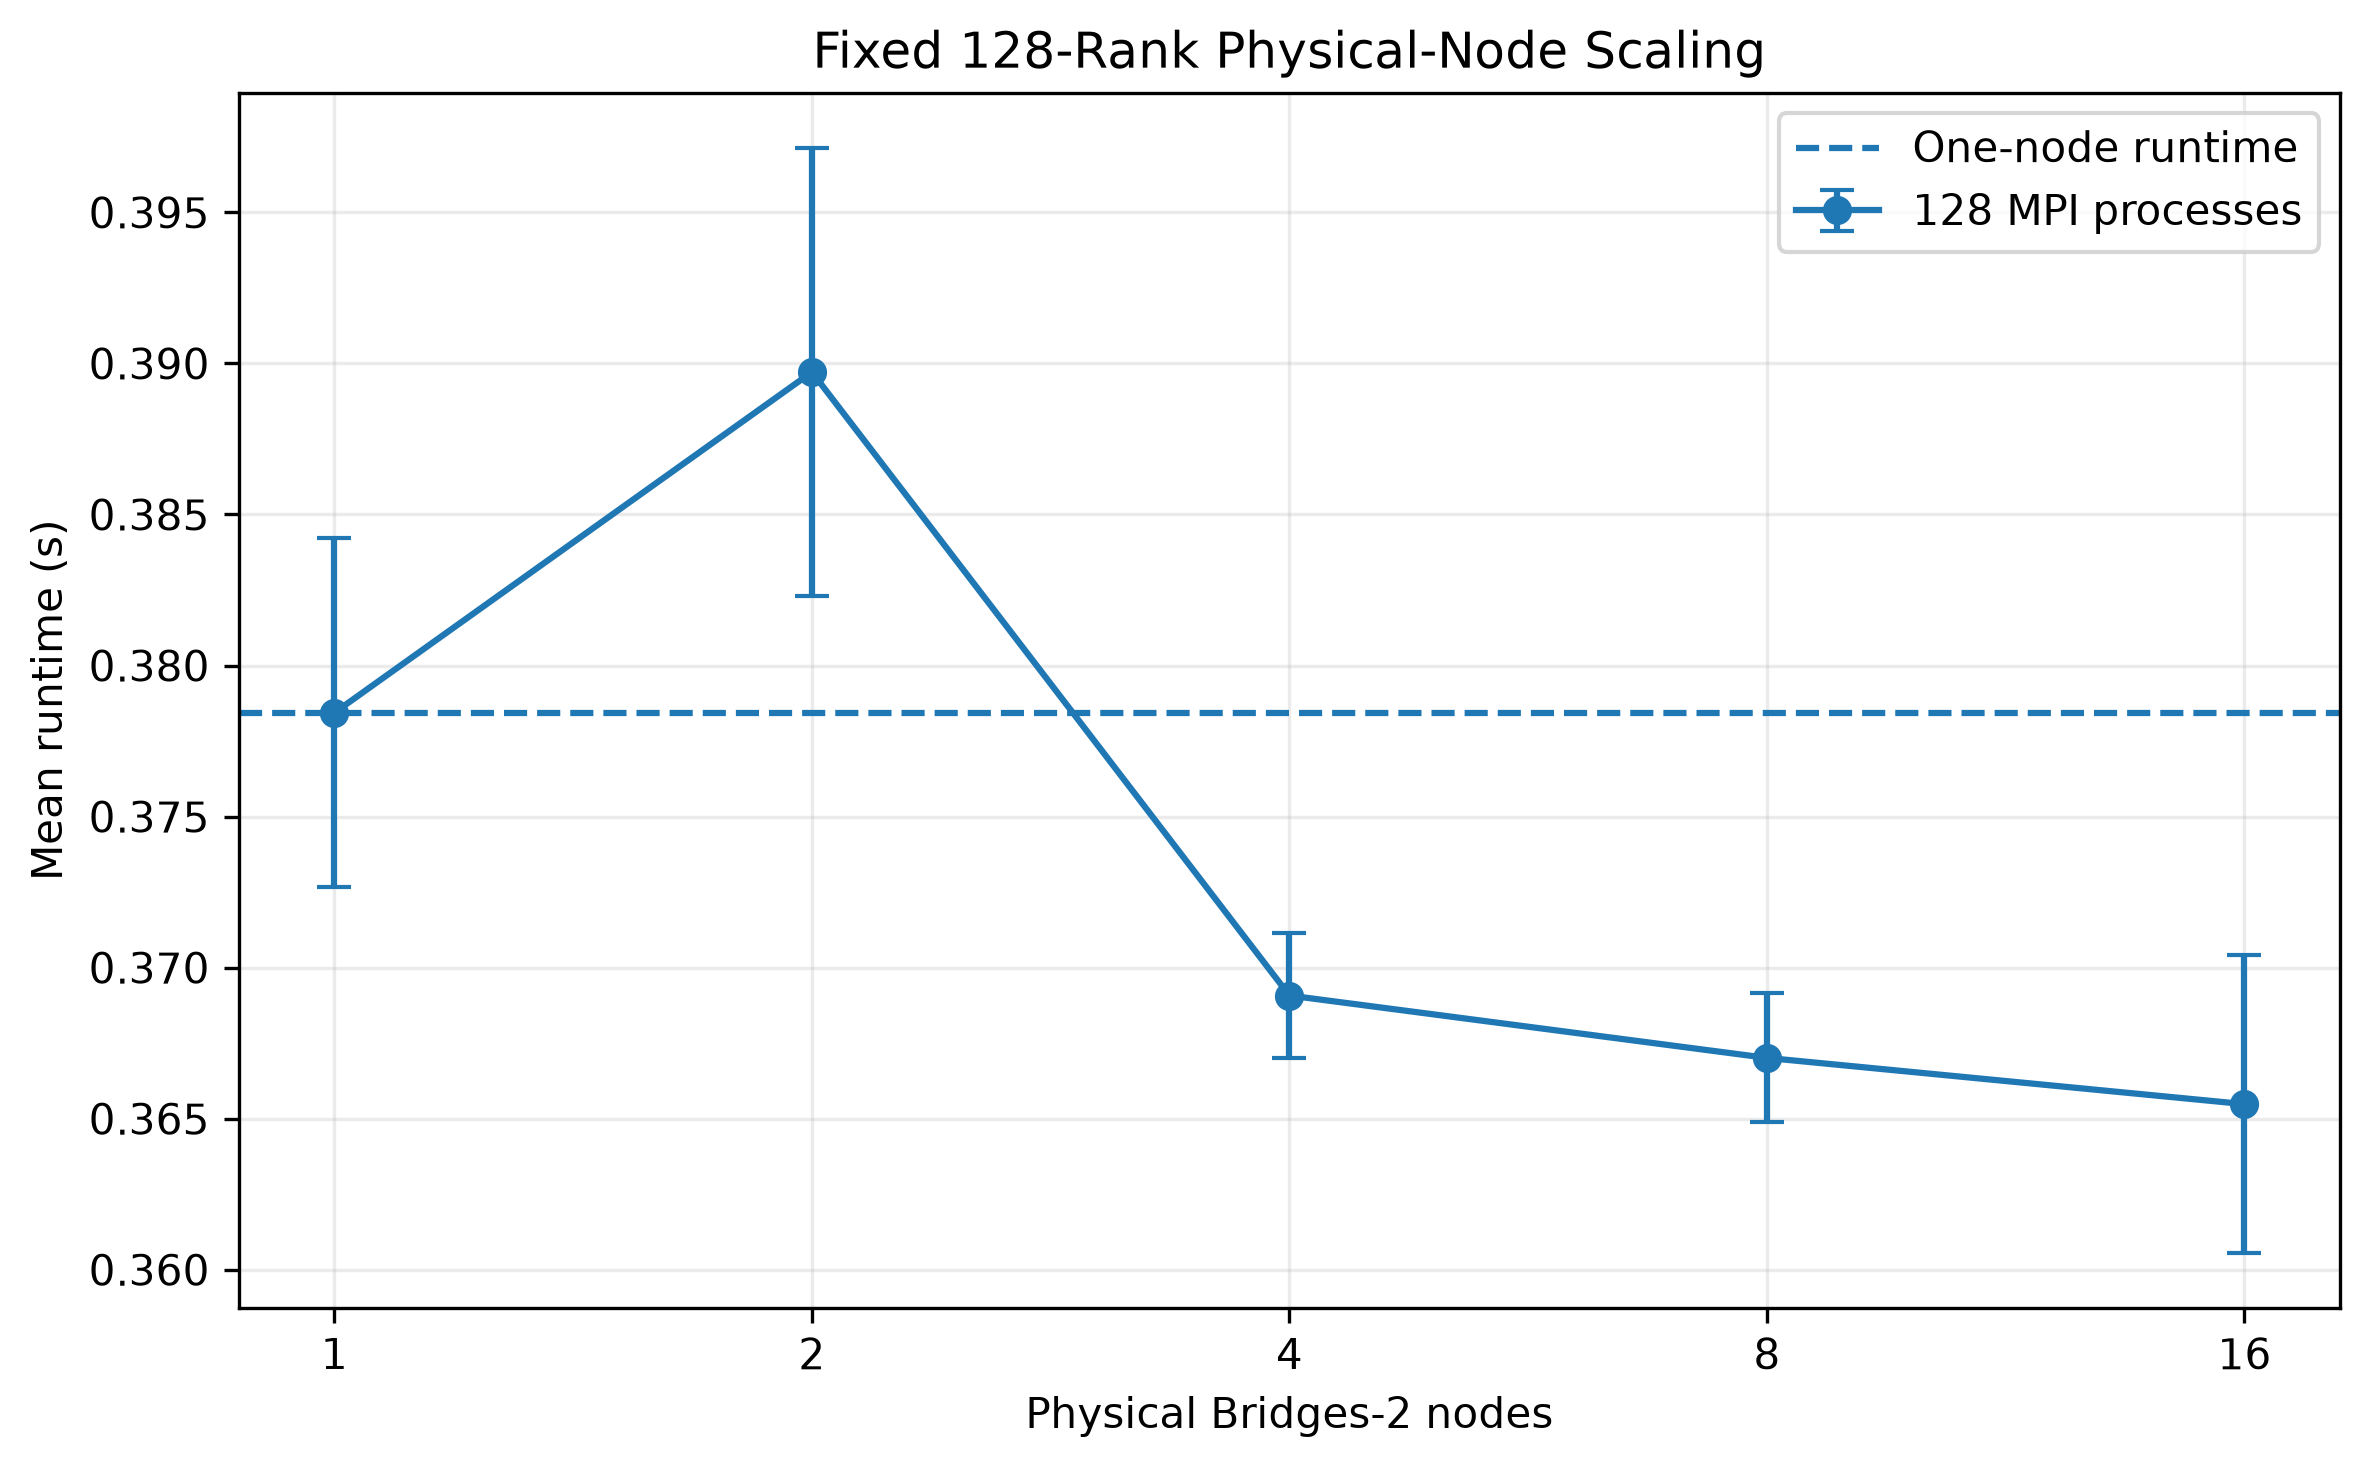
\includegraphics[width=0.90\textwidth]
    {figures/ninapro_fullcapacity_node_scaling.png}
    \caption{Physical-node scaling with the total MPI process count fixed
    at 128 ranks. The same 1,404-window, 986,310-pair workload was
    distributed across 1, 2, 4, 8, and 16 Bridges-2 Regular Memory nodes.
    The dashed line represents the measured 128-rank one-node runtime.}
    \label{fig:fullcapacity-node-scaling}
\end{figure}

The two-node configuration was approximately 2.98\% slower than the
one-node 128-rank configuration, while the four-, eight-, and sixteen-node
configurations were approximately 2.47\%, 3.02\%, and 3.42\% faster,
respectively. These differences are modest compared with the overall
process-count speedup and indicate that the larger workload was sufficient
to largely amortize inter-node communication overhead.


\subsubsection{Bridges-2 V100 Accelerator Benchmark}
\label{subsec:bridges-gpu-results}

The final accelerator experiment was performed on an exclusive Bridges-2 GPU
node equipped with NVIDIA Tesla V100-32GB GPUs. Qiskit Aer statevector
simulation was evaluated on both the CPU and a single V100 GPU. The Aer GPU
tensor-network method was also evaluated using the installed cuQuantum
software stack. Each configuration used one untimed warm-up followed by five
timed executions, and all resulting quantum-kernel matrices passed numerical
validation.

For the complete 102-sample, eight-qubit NinaPro kernel, the CPU statevector
backend required a mean runtime of 7.132028~s. The V100 statevector backend
required 7.210690~s, corresponding to a CPU-relative speedup of
\(0.989\times\). The GPU tensor-network backend required 8.277748~s,
corresponding to a CPU-relative speedup of \(0.862\times\).
Therefore, GPU acceleration did not improve performance for the complete
eight-qubit kernel workload.

\begin{table}[!htbp]
\centering
\caption{Final Bridges-2 backend comparison for the 102-sample,
eight-qubit NinaPro quantum kernel.}
\label{tab:bridges-gpu-kernel}

\begin{tabular}{lrrr}
\toprule
Backend &
Mean Runtime (s) &
Std. (s) &
Speedup vs. CPU \\
\midrule
CPU statevector &
7.132028 &
0.044020 &
1.000000 \\
V100 statevector &
7.210690 &
0.034396 &
0.989091 \\
V100 tensor network &
8.277748 &
0.026685 &
0.861590 \\
\bottomrule
\end{tabular}
\end{table}

\begin{figure}[H]
    \centering
    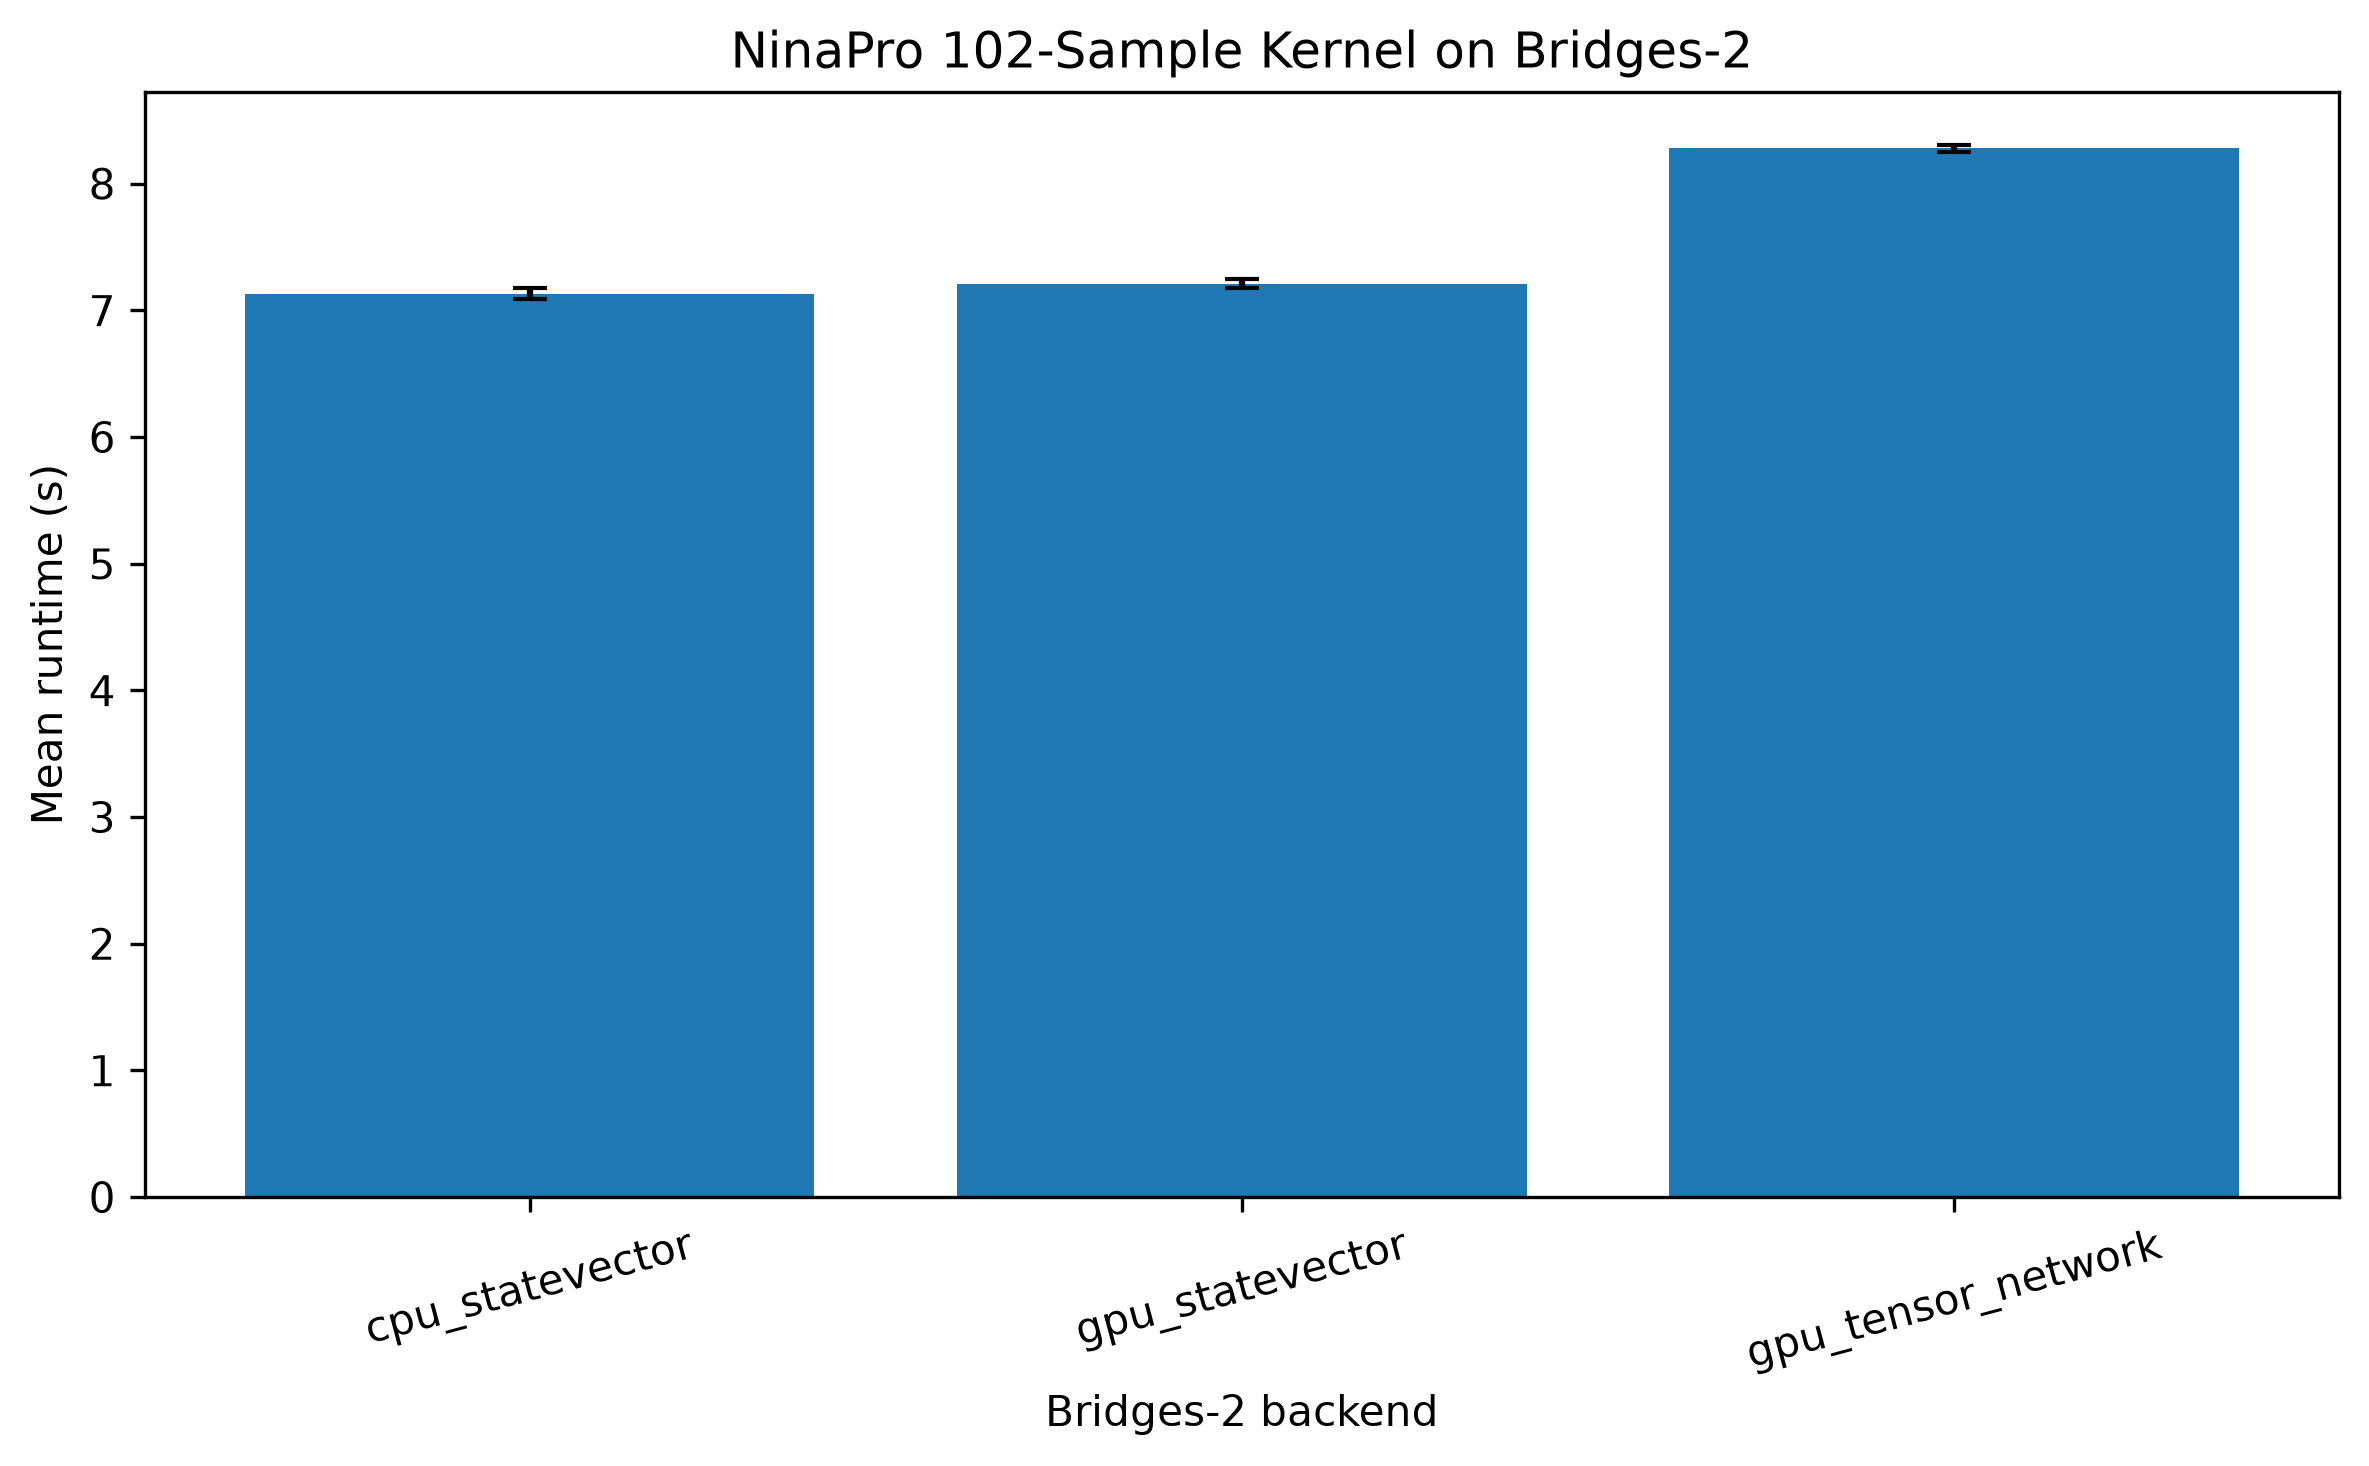
\includegraphics[width=0.90\textwidth]
    {figures/ninapro_bridges_backend_runtime.png}
    \caption{Mean runtime of the final 102-sample NinaPro quantum-kernel
    workload using Aer CPU statevector, V100 GPU statevector, and V100 GPU
    tensor-network simulation on Bridges-2. Error bars represent the standard
    deviation across five timed runs.}
    \label{fig:bridges-gpu-kernel}
\end{figure}

A separate controlled scaling experiment evaluated 4, 6, 8, 10, 12, 14,
and 16 qubits using eight deterministic feature vectors per circuit size.
CPU and V100 statevector runtimes remained similar from 4 through 14 qubits,
with the CPU retaining a small performance advantage at each of those tested
sizes. At 16 qubits, however, mean CPU runtime increased to 0.634693~s while
V100 statevector runtime was 0.594701~s, producing a measured
\(1.067\times\) GPU speedup.

The GPU tensor-network method remained slower than CPU statevector simulation
throughout the tested range. Its CPU-relative speedup decreased from
\(0.883\times\) at four qubits to \(0.769\times\) at sixteen qubits.

\begin{figure}[H]
    \centering
    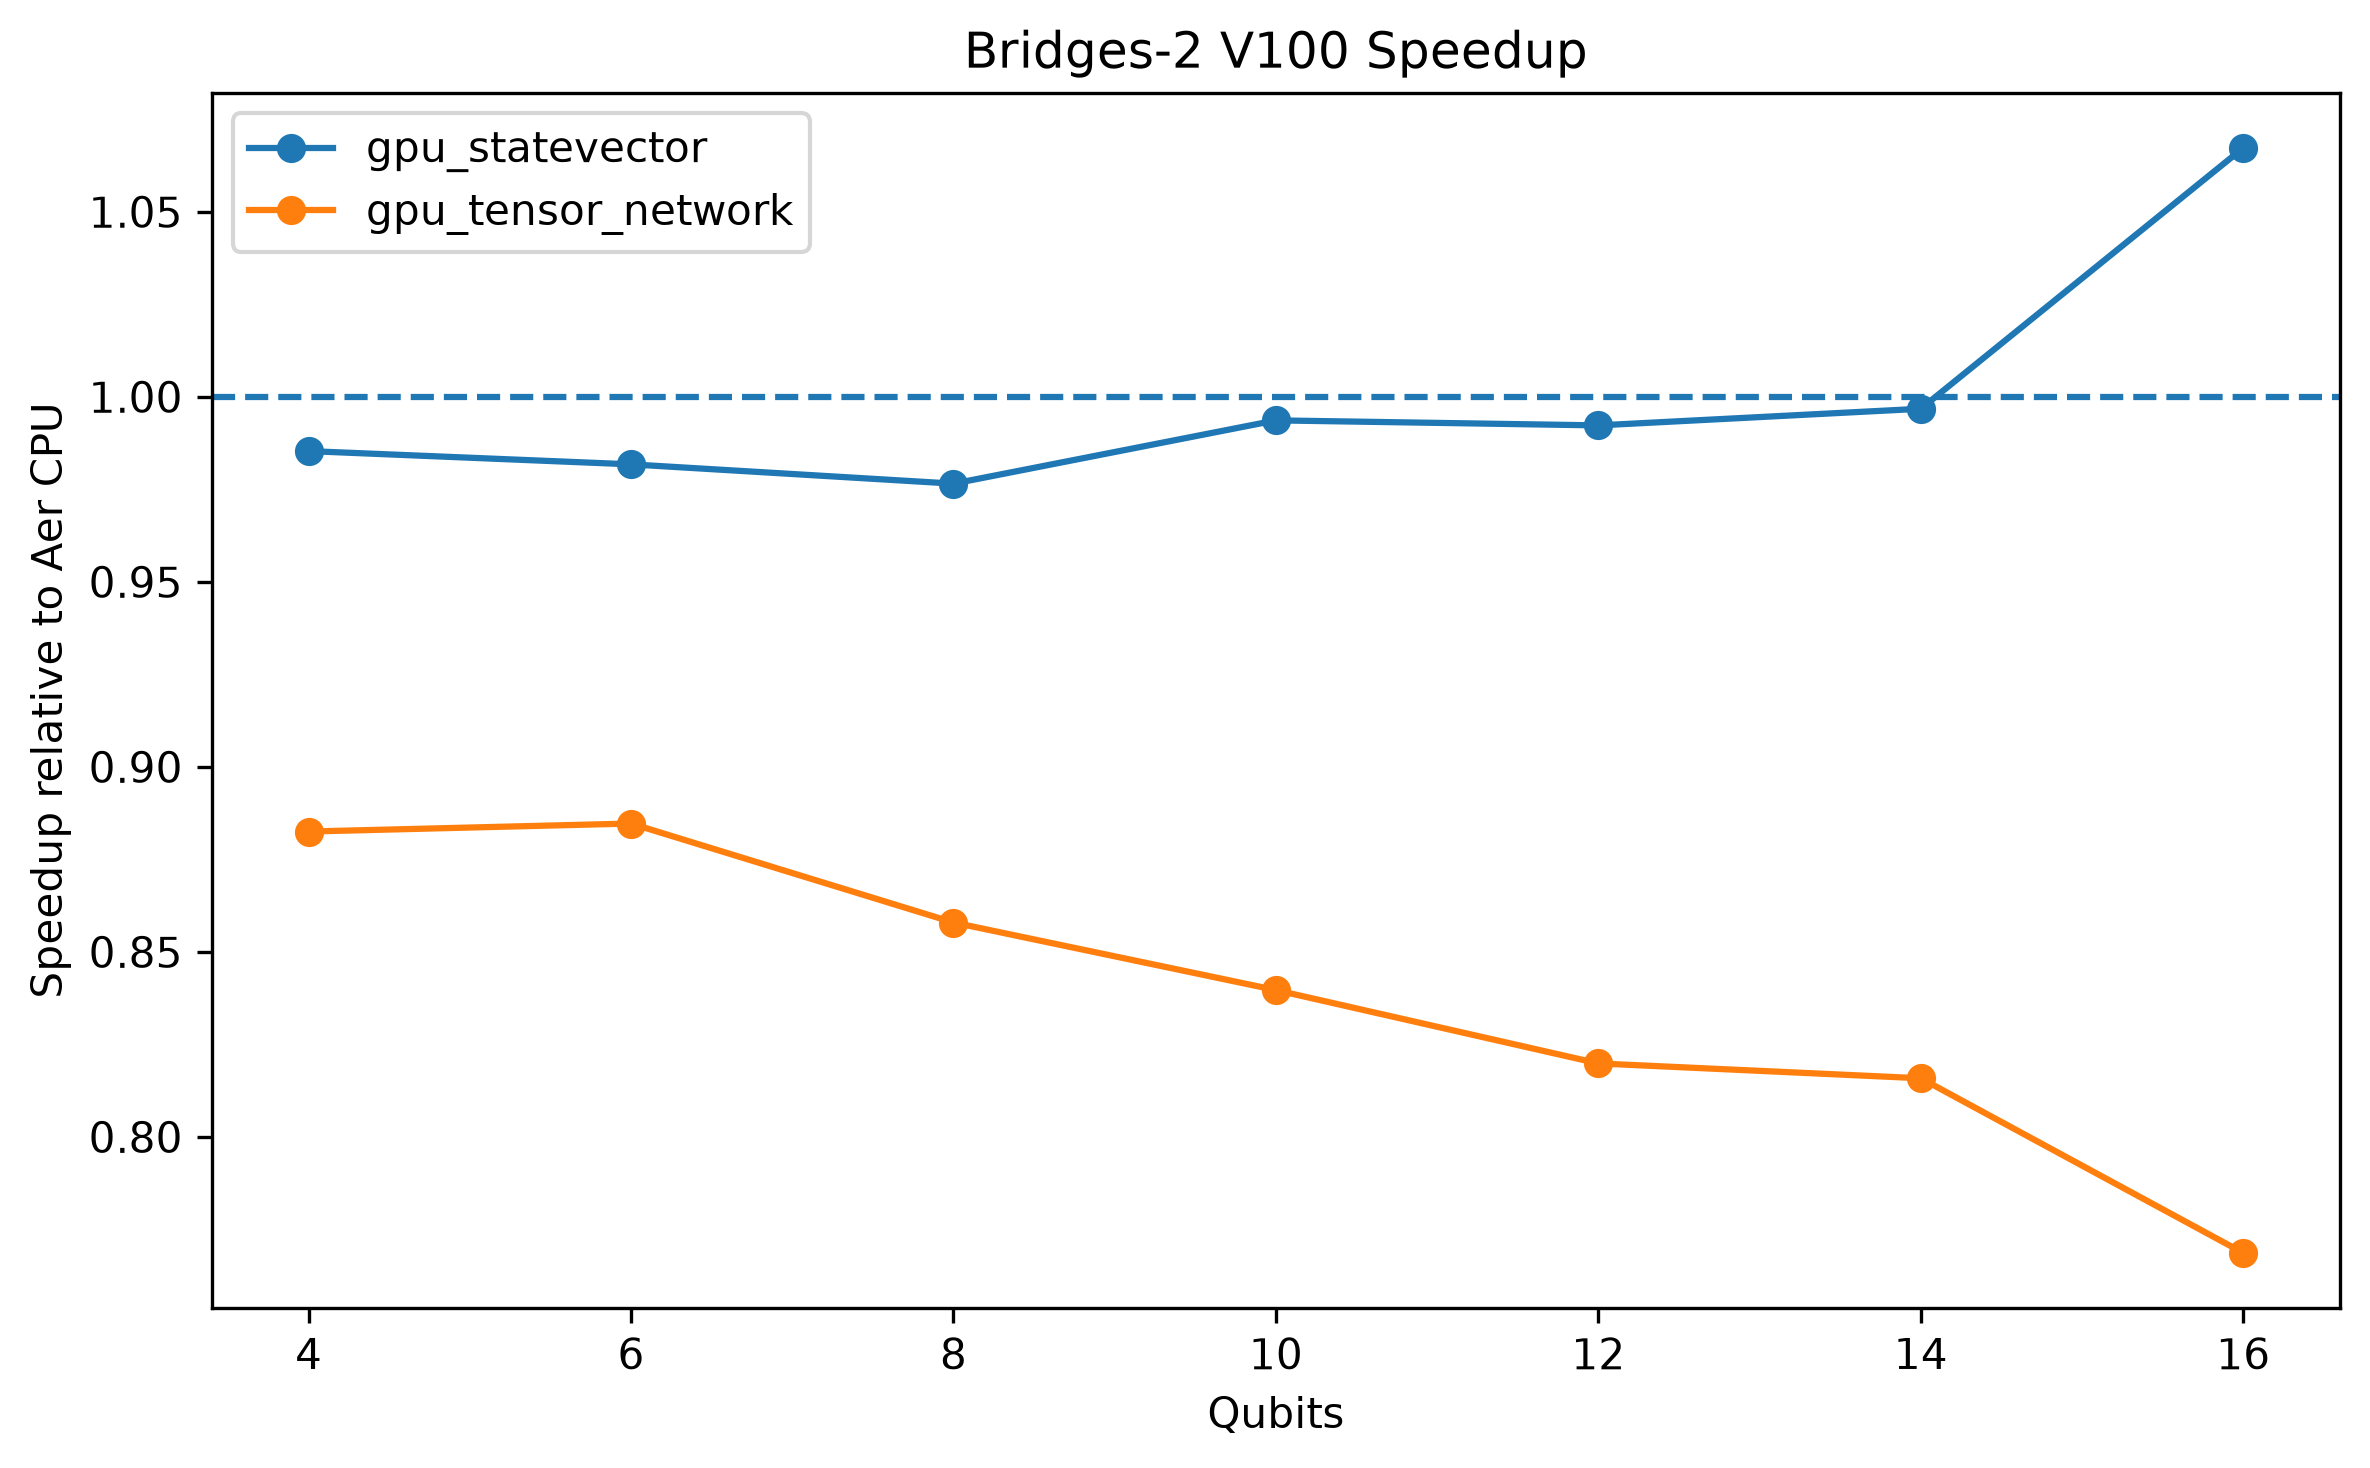
\includegraphics[width=0.90\textwidth]
    {figures/qubit_scaling_bridges_speedup.png}
    \caption{Bridges-2 V100 accelerator speedup relative to Aer CPU
    statevector simulation from 4 to 16 qubits. The dashed line at
    \(1.0\times\) represents equal CPU and GPU performance. V100 statevector
    simulation exceeds CPU performance only at the largest tested circuit
    size of 16 qubits.}
    \label{fig:bridges-gpu-speedup}
\end{figure}

These measurements indicate that accelerator overhead dominates the smaller
quantum-simulation workloads tested here. As the simulated statevector grows,
the relative cost of GPU overhead becomes less significant, and a performance
advantage begins to appear at the largest tested circuit size. Because the
experiment evaluates only discrete circuit sizes through 16 qubits, the
results identify a measured advantage at 16 qubits rather than establishing
a general CPU/GPU crossover threshold.


\section{Discussion}\label{sec:discussion}

\subsection{CPU and GPU Simulation Behavior}
\label{subsec:cpu-gpu-discussion}

The local CPU/GPU experiments demonstrate that accelerator use does not
automatically improve quantum-simulation performance. For the complete
eight-qubit NinaPro quantum-kernel workload, the CPU implementation completed
the benchmark faster than the local RTX 2080 SUPER GPU implementation. In
contrast, the controlled qubit-scaling experiment showed a change in relative
performance at 16 qubits, where the GPU completed the tested workload
approximately $2.44\times$ faster than the CPU.

These results suggest that the usefulness of GPU acceleration depends strongly
on workload size. At lower qubit counts, simulator setup, kernel launch, memory
transfer, and other accelerator overheads may represent a substantial fraction
of total runtime. As the size of the simulated state space increases, the
amount of parallel numerical work also increases, allowing GPU execution to
become more competitive.

The measured crossover should be interpreted as specific to the tested
hardware, circuit construction, simulator implementation, and benchmark
configuration. In particular, the CPU and GPU paths use different simulation
software, and the local GPU measurements were obtained using an NVIDIA
GeForce RTX 2080 SUPER. The results therefore characterize the behavior of the
implemented workflow rather than establishing a universal qubit threshold at
which GPU simulation becomes preferable.

The comparatively large runtime variation observed for the 16-qubit CPU
measurement also warrants caution when interpreting the exact magnitude of the
measured speedup. The important result is the observed change in relative
CPU/GPU behavior as circuit size increased, rather than the identification of a
fixed crossover point.

The Bridges-2 accelerator experiment reinforces the workload-size dependence
observed during local GPU testing. For the complete eight-qubit NinaPro
kernel, V100 statevector simulation did not outperform CPU statevector
simulation, with mean runtimes of 7.210690~s and 7.132028~s, respectively.
This indicates that the computational work at eight qubits remained too small
to offset GPU execution overhead.

In the controlled qubit-scaling experiment, CPU and V100 statevector
performance remained close from 4 through 14 qubits. At the largest tested
size of 16 qubits, the V100 statevector backend became faster, producing a
measured \(1.067\times\) speedup relative to the Aer CPU backend. This result
is consistent with the expectation that accelerator hardware becomes more
useful as statevector size and simulation work increase.

The GPU tensor-network method did not provide a performance advantage for the
tested circuits. Tensor-network performance depends strongly on circuit
structure, entanglement, contraction strategy, and simulation size; therefore,
the observed result should not be interpreted as a general comparison between
tensor-network and statevector simulation. Rather, the shallow manual
ZZFeatureMap circuits and modest 4--16-qubit range tested here did not provide
a workload for which the additional tensor-network machinery produced a
runtime benefit.

The Bridges-2 results should also be interpreted separately from the local
RTX 2080 SUPER experiment. The two environments use different hardware and
simulation software stacks, so absolute runtime values are not treated as a
direct GPU-to-GPU hardware comparison. Instead, both experiments are used to
evaluate how accelerator usefulness changes as the quantum simulation workload
increases.

\subsection{Numerical Consistency Across Simulation Backends}
\label{subsec:numerical-discussion}

The CPU and GPU implementations produced closely matching quantum-kernel
matrices, with a maximum absolute element-wise difference of approximately
$4.77\times10^{-7}$ and a mean absolute difference of approximately
$5.04\times10^{-9}$. Both implementations also satisfied the expected kernel
properties, including symmetry, a unit diagonal, finite values, and entries
within the interval $[0,1]$.

This numerical agreement is important because the GPU implementation is not
simply a different execution mode of the same simulator. The manually
constructed Qiskit feature-map circuit is translated into a separate qsim-based
GPU representation. Agreement between the two resulting kernel matrices
therefore provides evidence that the translation preserves the intended
quantum-kernel computation within normal floating-point numerical variation.

The validation also supports the use of the same biomedical feature vectors
across the subsequent performance experiments. Performance comparisons are
therefore based on implementations that have first been checked for numerical
consistency rather than on runtime alone.


\subsection{Effect of Depolarizing Noise}
\label{subsec:noise-discussion}

The controlled depolarizing-noise experiment produced a monotonic decrease in
mean state fidelity as the noise probability increased from $p=0.001$ to
$p=0.050$. Mean fidelity decreased from approximately 0.99996 to approximately
0.99804 over the tested range, while the variation in fidelity across the
102 samples increased with noise strength.

Although the numerical decrease in mean fidelity is relatively small, the
trend is consistent across the tested noise levels. These results demonstrate
that the implemented workflow can quantify degradation of the encoded NinaPro
states under a controlled quantum-noise model. They should not, however, be
interpreted as a characterization of a particular physical quantum processor.
The experiment uses a simplified depolarizing model applied within classical
simulation.

Mean runtime remained close to 0.042 seconds per sample across all five noise
strengths. Within the tested range, increasing the depolarizing probability
therefore changed the resulting quantum states without producing a comparable
increase in simulation time. This result is specific to the eight-qubit
density-matrix workload and the tested Aer configuration.

The quantum-noise experiment is also distinct from the differential-privacy
experiments conducted during earlier stages of the broader DREU-QIS project.
The parameter $p$ represents simulated quantum gate noise, whereas the
differential-privacy parameter $\epsilon$ controls a privacy mechanism. The two
parameters describe different experimental phenomena and are not directly
comparable.


\subsection{MPI Scaling and HPC Execution}
\label{subsec:mpi-discussion}

The Bridges-2 experiments demonstrate that the pairwise quantum-kernel
workload can be parallelized effectively using workload-level MPI. In the
original 102-sample strong-scaling experiment, mean runtime decreased from
0.168016~s with one process to 0.024862~s with eight processes, producing a
measured \(6.76\times\) speedup. Parallel efficiency remained 99.62\% at two
processes, 94.48\% at four processes, and 84.47\% at eight processes.

The accompanying weak-scaling experiment maintained approximately 5200
kernel-pair evaluations per rank. Calculated efficiencies exceeded 100\%
because the complete timed workflow includes both pair evaluation and
quantum-state encoding, and the amount of state-encoding work assigned to each
rank decreases as process count increases. These values should therefore be
interpreted as kernel-pair weak scaling of the implemented workflow rather
than conventional superlinear scaling of a strictly constant workload per
process.

The first multi-node topology experiment used the small 102-sample workload.
At matched process counts, distributing ranks across multiple physical nodes
increased runtime, particularly at sixteen and thirty-two processes. This
indicated that inter-node communication represented a significant fraction of
the total execution time when only 5253 kernel-pair evaluations were available.

Increasing the workload to 714 distinct real EMG windows and 255,255
kernel-pair evaluations substantially changed this behavior. Matched
single-node and multi-node configurations differed by less than 0.4\% at
8, 16, and 32 MPI processes, indicating that the increased computation was
sufficient to largely amortize the inter-node communication cost.

The final full-capacity experiment extended this trend using 1,404 distinct
non-overlapping real EMG windows and 986,310 kernel pairs. On a single node,
runtime decreased from 4.198034~s with one MPI process to 0.378437~s with
128 processes, corresponding to an \(11.093\times\) speedup. Parallel
efficiency, however, declined to 8.67\% at 128 processes, demonstrating
substantial diminishing returns at high process counts.

The fixed-128-rank topology experiment provides the clearest isolation of
physical-node effects. Moving from one to two nodes increased runtime by
approximately 2.98\%, while distributing the same 128 ranks across four,
eight, and sixteen nodes reduced mean runtime by approximately 2.47\%,
3.02\%, and 3.42\%, respectively, relative to the one-node configuration.
The fastest measured topology used sixteen nodes and eight ranks per node,
with a mean runtime of 0.365481~s.

The modest size of these topology differences compared with the much larger
process-count speedup is important. The results do not show that adding
physical nodes alone produces large acceleration. Rather, they show that once
the workload becomes sufficiently large, the cost of inter-node communication
can be amortized to the point that distributing a fixed number of ranks across
several physical nodes is competitive with, and in some tested configurations
slightly faster than, concentrating all ranks on one node.

Across the 102-, 714-, and 1,404-window experiments, the overall pattern is
therefore consistent: workload size strongly affects the usefulness of
distributed-memory execution. Small workloads expose communication overhead
more clearly, while larger workloads provide enough independent pairwise work
to make multi-node execution increasingly practical. At the same time, the
declining parallel efficiency observed at high MPI process counts shows that
communication, synchronization, state exchange, result gathering, and other
non-parallel costs ultimately limit strong-scaling performance.


\subsection{Biomedical Workload and Scope}
\label{subsec:biomedical-discussion}

The use of NinaPro DB2 provides a real biomedical signal-processing workload
for evaluating the computational framework. Rather than benchmarking only
randomly generated numerical vectors or synthetic circuit inputs, the final
kernel is constructed from features derived from recorded surface-EMG signals.

The present study does not attempt to evaluate gesture-classification accuracy
or clinical performance. Gesture labels are used to identify the corresponding
recording segments and construct a reproducible set of samples, but no
classifier-performance claim is made from the resulting quantum kernel.

Similarly, the use of eight PCA-derived features is primarily a computational
design choice that allows the processed biomedical data to be mapped directly
to an eight-qubit feature map. The experiment therefore evaluates the
computational behavior of a quantum-kernel workflow on biomedical data rather
than demonstrating that eight quantum features represent an optimal
classification model.


\subsection{Limitations}\label{subsec:limitations}

Several limitations should be considered when interpreting the results.

First, the biomedical benchmark uses a single NinaPro DB2 subject and a single
exercise/acquisition file. The primary workload contains one selected window
from each of 17 gesture classes and six repetitions. The balanced larger
workload contains seven distinct non-overlapping windows from each of those
gesture--repetition segments, while the final full-capacity workload contains
every complete non-overlapping 512-sample window available from those same
segments, for a total of 1,404 windows. These larger workloads increase the
amount of real recorded EMG data used for computation but do not represent
additional subjects or independent gesture repetitions, and they should not
be interpreted as representative of the complete NinaPro DB2 population.

Second, larger weak-scaling workloads reuse the same 102 processed feature
vectors deterministically. The 144-, 204-, and 289-sample workloads therefore
represent increased computational workloads rather than additional independent
biomedical observations.

Third, all quantum results in this study are produced through classical quantum
simulation. No claim of quantum computational advantage is made, and the
measured CPU, GPU, and MPI behavior reflects the cost of simulating the quantum
workload on classical hardware.

Fourth, the local CPU and GPU implementations use different simulation
software. Although numerical agreement was explicitly validated, performance
differences reflect both the underlying hardware and the implementation details
of the respective simulators.

Fifth, the depolarizing-noise experiment uses a controlled simulation model and
does not reproduce the complete error characteristics of a specific physical
quantum processor.

Finally, the weak-scaling experiment maintains an approximately constant
number of kernel-pair calculations per MPI rank rather than a strictly
constant amount of total timed work per rank. The timed workflow also includes
quantum-state encoding, state exchange, and result gathering. The resulting
weak-scaling efficiencies above 100\% should therefore be interpreted in the
context of this workload design rather than as evidence of universally
superlinear MPI scaling.

The MPI experiments remain limited in dataset scope despite the increased
computational workload. The primary kernel contains 102 samples and 5253
upper-triangular pair evaluations, the balanced larger workload contains
714 distinct windows and 255,255 pairs, and the final full-capacity workload
contains 1,404 distinct non-overlapping windows and 986,310 pairs. All three
workloads are derived from the same Subject 1, Exercise 1, Acquisition 1
recording.

Multi-node execution was evaluated through 16 Bridges-2 Regular Memory nodes
and 128 MPI processes. The observed topology behavior should therefore not be
generalized directly to the complete NinaPro DB2 dataset, substantially
higher-qubit simulations, larger node counts, or different communication
patterns. The MPI implementation parallelizes independent quantum-state
encoding and quantum-kernel tasks; it does not distribute a single quantum
statevector across multiple nodes.


\section{Conclusion}\label{sec:conclusion}

This work developed and evaluated a reproducible high-performance computing
workflow for simulated quantum-kernel calculations using biomedical EMG data.
The final experimental pipeline connects NinaPro DB2 preprocessing, classical
feature extraction, dimensionality reduction, manual quantum feature-map
construction, quantum-kernel evaluation, CPU and GPU simulation, controlled
noise characterization, and MPI-based workload distribution.

The NinaPro benchmark produced 102 eight-dimensional quantum feature vectors
derived from 12-channel surface-EMG recordings. These vectors were used to
construct a complete $102\times102$ quantum-kernel workload based on an
eight-qubit manually constructed feature map. Independent CPU and CUDA-capable
GPU implementations produced numerically consistent kernel matrices, with a
maximum absolute difference of approximately $4.77\times10^{-7}$.

Local performance measurements showed that the CPU completed the full
eight-qubit NinaPro kernel benchmark faster than the GPU. However, controlled
qubit-scaling experiments demonstrated that the relative performance changed as
circuit size increased. At 16 qubits, the local GPU completed the tested
simulation approximately $2.44\times$ faster than the CPU. These measurements
show that accelerator benefit depends on workload size and that small quantum
simulations do not necessarily provide enough computational work to offset GPU
overhead.

The controlled depolarizing-noise experiment further demonstrated that the
framework can evaluate changes in simulated quantum-state fidelity. Mean
fidelity decreased monotonically across the tested noise strengths, from
approximately 0.99996 at $p=0.001$ to approximately 0.99804 at $p=0.050$,
while average simulation runtime remained close to 0.042 seconds per sample.

The project also demonstrated distributed-memory execution on the Bridges-2
high-performance computing system. For the fixed 102-sample NinaPro workload,
single-node strong scaling reduced mean runtime from 0.168016~s with one MPI
process to 0.024862~s with eight processes, corresponding to a
\(6.758\times\) speedup and 84.47\% parallel efficiency. Weak-scaling
experiments further demonstrated that the independent pairwise structure of
the quantum kernel can be distributed across MPI ranks, although calculated
efficiencies above 100\% reflect the mixed state-encoding and kernel-pair work
contained in the timed workflow.

A first multi-node experiment using the 102-sample workload showed measurable
communication overhead when matched process counts were spread across
additional nodes. Increasing the workload to 714 distinct real EMG windows and
255,255 kernel pairs largely removed this penalty, with matched single-node
and multi-node runtimes differing by less than 0.4\%.

The final full-capacity MPI experiment used 1,404 distinct non-overlapping
real EMG windows and 986,310 kernel pairs. On one node, increasing process
count from one to 128 reduced mean runtime from 4.198034~s to 0.378437~s,
corresponding to an \(11.093\times\) speedup. When the same 128 MPI ranks
were distributed across 16 Bridges-2 nodes, mean runtime decreased further
to 0.365481~s, producing the fastest measured configuration and an overall
\(11.486\times\) speedup relative to the single-process baseline.

These results show that workload-level MPI can effectively exploit the
independent pairwise structure of quantum-kernel construction, while also
demonstrating two important scaling limits. First, increasing MPI process count
produces diminishing returns as communication and synchronization overhead
become more significant. Second, the effect of distributing ranks across
physical nodes depends strongly on workload size: multi-node overhead was
clearly visible for the smallest workload, approximately neutral for the
714-window workload, and modestly favorable in several configurations of the
1,404-window workload.

The final Bridges-2 accelerator experiment additionally evaluated Aer CPU
statevector, V100 GPU statevector, and V100 GPU tensor-network simulation.
For the complete eight-qubit NinaPro kernel, accelerator overhead prevented
either GPU configuration from outperforming CPU execution. In the controlled
qubit-scaling experiment, however, V100 statevector simulation became faster
than CPU statevector simulation at the largest tested size of 16 qubits,
achieving a measured \(1.067\times\) speedup. These results further demonstrate
that accelerator effectiveness depends strongly on simulation scale and
workload characteristics.

Overall, the work demonstrates a complete experimental path from real biomedical
signals to a simulated quantum-kernel workload that can be validated and
benchmarked across CPU, GPU, noisy-simulation, and distributed HPC
configurations. The results do not establish quantum advantage or biomedical
classification superiority; rather, they characterize the computational
requirements and scaling behavior that must be understood when developing
larger quantum-machine-learning simulation studies.

\section*{Author Contributions}

Kyle Hartness developed the HPC benchmarking and parallelization workflow,
implemented the NinaPro biomedical workload, developed and validated the local
CPU and GPU quantum-kernel simulation paths, performed the qubit-scaling and
depolarizing-noise experiments, developed the MPI strong-, weak-, and
multi-node scaling benchmarks, designed and executed the 714-window and
1,404-window real-data MPI extensions through 128 MPI ranks and 16 physical
Bridges-2 nodes, configured and evaluated the Bridges-2 V100 accelerator
environment, and analyzed the resulting performance data.

Edmund Bombardieri contributed to the quantum-computing component of the
broader DREU-QIS project, including development and evaluation of the quantum
feature-map and quantum-kernel methodology that informed the workload used in
this study.

Sofia Furda contributed to the broader project architecture, including the
privacy-aware and distributed-processing components developed in parallel with
the HPC benchmarking work.

All authors reviewed the project direction and contributed to the broader
DREU-QIS research effort.

\section*{Acknowledgements}

%The authors thank Rutal Mahajan for mentorship, technical guidance, and support
%throughout the DREU-QIS research project.

This work used Bridges-2 at Pittsburgh Supercomputing Center through allocation
cis260310p from the Advanced Cyberinfrastructure Coordination
Ecosystem: Services \& Support (ACCESS) program, which is supported by National
Science Foundation grants \#2138259, \#2138286, \#2138307, \#2137603, and
\#2138296.

This material is based upon work supported by the National Science Foundation
under Award No. 2620473.

\section*{Funding}

This work was supported by the National Science Foundation through the
DREU-QIS program under Award No. 2620473.

\section*{Data Availability}

The biomedical workload used in this study was derived from the publicly
available NinaPro DB2 surface-electromyography dataset. Raw NinaPro data are not
redistributed with the QuantumHPC repository. The preprocessing and benchmark
code required to construct the experimental workload from an appropriately
obtained NinaPro DB2 file is included in the project repository.

\section*{Code Availability}

The software developed for this project is maintained in the public QuantumHPC
project repository:

\url{https://github.com/DREU-QIS-2026/Quantum-Enhanced-Privacy-Preserving-NLP-for-Clinical-Text-De-Identification}

The repository includes the NinaPro preprocessing pipeline, manual quantum
feature-map implementation, quantum-kernel evaluation code, CPU and GPU
simulation interfaces, depolarizing-noise benchmark, MPI strong- and weak-scaling
benchmarks, SLURM execution scripts, saved experimental results, and analysis
utilities used to generate the reported results.

\section*{Competing Interests}

The authors declare no competing interests.

\backmatter

\bibliography{sn-bibliography}% common bib file
%% if required, the content of .bbl file can be included here once bbl is generated
%%\input sn-article.bbl

\end{document}